\documentclass{beamer}

\mode<presentation>
{
  \usetheme{metropolis}      % or try Darmstadt, Madrid, Warsaw, ...
  \usecolortheme{rose} % or try albatross, beaver, crane, ...
  \usefonttheme{structurebold}  % or try serif, structurebold, ...
  \setbeamertemplate{navigation symbols}{}
  \setbeamertemplate{caption}[numbered]
  \setbeamertemplate{itemize items}[square]
}
\usepackage[english]{babel}
\usepackage[utf8]{inputenc}
\usepackage{lmodern}
\usepackage[T1]{fontenc} 
\usepackage{microtype}
\usepackage{inconsolata}
%\usepackage{fontspec}
\usepackage{graphicx}
\usepackage{caption}
\usepackage[percent]{overpic}
\usepackage{csquotes}

\usepackage{amsmath}
\usepackage{amsfonts}
\usepackage{amssymb}
\usepackage{amsthm}
\usepackage{mathrsfs}

\usepackage{systeme}

\usepackage{tikz}
\usetikzlibrary{overlay-beamer-styles}
\usetikzlibrary{calc,trees,positioning,arrows,fit,shapes}
\usetikzlibrary{decorations.pathreplacing}
\usetikzlibrary{patterns}
\usetikzlibrary{backgrounds}

\usepackage[backend=biber,bibencoding=utf8,style=ieee]{biblatex}
\addbibresource{references.bib}
\newcommand{\Av}[1]{\textsf{Av}\left(#1\right)}
\newcommand{\Avn}[2]{\textsf{Av}_{#1}\left(#2\right)}
\newcommand{\Co}[1]{\textsf{Co}\left(#1\right)}
\newcommand{\contains}[2]{#2 \preceq #1}
\newcommand{\set}[1]{\left\{#1\right\}}
\newcommand{\cset}[2]{\left\{#1 \mid #2\right\}}
\newcommand{\N}{\mathbb{N}}
\newcommand{\Z}{\mathbb{Z}}
\newcommand{\Q}{\mathbb{Q}}
\newcommand{\R}{\mathbb{R}}
\newcommand{\C}{\mathbb{C}}
\newcommand\at[2]{\left.#1\right|_{#2}}
\newcommand{\gridN}{\raisebox{-2pt}{\tikz{\draw[step=0.2] (0,0) grid (.2,.4);}}}
\newcommand{\gridD}{\raisebox{-2pt}{\tikz{\fill[gray!50] (0,0) rectangle (0.2,0.2);\draw[step=0.2] (0,0) grid (.2,.4);}}}
\newcommand{\gridU}{\raisebox{-2pt}{\tikz{\fill[gray!50] (0,0.2) rectangle (0.2,0.4);\draw[step=0.2] (0,0) grid (.2,.4);}}}

\newcommand\ptedge[4]{
  \draw ($#1 + (0.5, -1.3) + #2$)..%
  controls ($#1 + #2 + (0.5, -1.3) + (0, -1)$)%
  and ($#3 + #4 + (0, 1) + (0.5, -0.3)$)..%
  ($#3 + #4 + (0.5, -0.3)$);
}

\newcommand{\point}[1]{%
    \begin{tikzpicture}
        \filldraw (0, 0) circle (#1);
    \end{tikzpicture}
}

\algnewcommand\algorithmicforeach{\textbf{for each}}
\algdef{S}[FOR]{ForEach}[1]{\algorithmicforeach\ #1\ \algorithmicdo}
\newcommand{\algorithmiccontinue}{\textbf{continue}}

% Paper notation : Change here should change everything in paper
\newcommand{\st}[1]{\textsf{st}\left(#1\right)}
\newcommand{\sseq}[2]{\Xi(#1,#2)}
\newcommand{\spec}[1]{\check{\mathcal{#1}}}
\newcommand{\specset}{\mathfrak{A}}
\newcommand{\specg}[1]{\mathfrak{G}\left(\check{\mathcal{#1}}\right)}
\newcommand{\sclsi}[2]{\mathcal{#1}^{\left(#2\right)}}
\newcommand{\src}{\textsf{src}}
\newcommand{\dst}{\textsf{dst}}
\newcommand{\op}{\textsf{op}}

\newcommand{\css}{\texttt{CombSpecSearcher}}
\newcommand{\tsc}{\texttt{TileScope}}

\newcommand{\sym}{\textsf{sym}}

\newcommand{\rev}{\textsf{r}}
\newcommand{\inv}{\textsf{i}}

\newcommand{\wordseq}[2]{#1_1 #1_2 \dotsm #1_{#2}}
\newcommand{\wordrev}[2]{#1_{#2} #1_{#2 - 1} \dotsm #1_1}
\newcommand{\wordidx}[3]{#1_{#2_1} #1_{#2_2} \dotsm #1_{#2_{#3}}}
\newcommand{\perm}[2]{\wordseq{#1}{#2}}
\newcommand{\setn}{\set{1,2,\dotsc,n}}
\newcommand{\idxset}[2]{\set{#1_1,#1_2,\dotsc,#1_{#2}}}
\newcommand{\idxord}[2]{#1_1 < #1_2 < \dotsm < #1_{#2}}

\newcommand{\sort}{\textsf{sort}}




\title[Automated Bijections]{Automated Bijections\\with Combinatorial Exploration}
\author[Jón Steinn Elíasson]{Jón Steinn Elíasson}
\institute[Reykjavik University]{Reykjavík University}
\date{\today}

\begin{document}

{
\newcommand{\backgroundart}{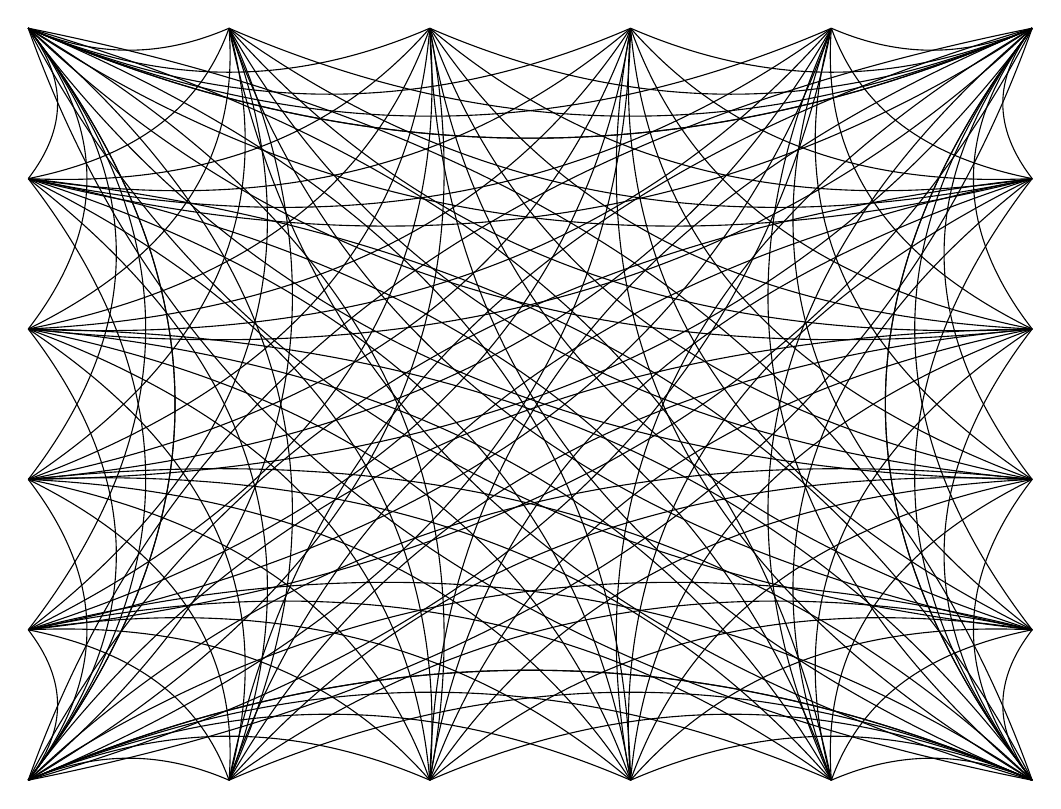
\begin{tikzpicture}[yscale=0.955,xscale=1.275]
    \foreach \x in {0,2,...,10} {%
        \foreach \y in {0,2,...,10} {%
            \draw (\x,0)  to [bend right] (0,\y);
            \draw (\x,10) to [bend left] (0,10-\y);
            \draw (\x,10) to [bend right] (10,10-\y);
            \draw (10-\x,0) to[bend left] (10,10-\y);
        }
    }
\end{tikzpicture}}
\usebackgroundtemplate{\tikz[remember picture,overlay,opacity=0.04,inner sep=0] \node at (current page.center) {\backgroundart};}

\begin{frame}
    \titlepage
    \tikz [remember picture,overlay] \node at ([yshift=8cm,xshift=4.8cm]current page.south) {
\includegraphics[scale=0.5]{graphics/ru-logo.eps}};
\end{frame}
}
\begin{frame}{Outline}
  \tableofcontents
\end{frame}

\section{Introduction}
\begin{frame}{Introduction}
    \begin{itemize}
        \item<1-> Combinatorics
        \subitems{%
            \item Discrete structures
            \item Enumerative combinatorics
            \item Permutation patterns
            \subsubitems{%
                \item First enumeration \authcite{MacMahon}
                \item Surge of interest \authcite{knuth:aocp1}
                \item First bijection \authcite{simionandschmidt}
            }
        }
        \item<2-> Automation
        \subitems{%
            \item Earliest enumeration example \authcite{Zeilberger1998EnumerationSA}
            \item Combinatorial Exploration \authcite{BeanPhd:phd}
            \item The translation method \authcite{wood_zeilberger}
        }
        \item<3-> My work
        \subitems{%
            \item Use Combinatorial Exploration to find bijections
            \item 189 bijections found
        }
    \end{itemize}
\end{frame}

\section{Background}
\begin{frame}{Combinatorial class}
    \begin{block}{Definition}<1->
        A \emph{combinatorial class} is a set $\mathcal{C}$ and a size function $\mathcal{C} \mapsto \N = \set{0,1,2,\dotsc}$ such that
\[
    \mathcal{C}_n = \cset{c \in \mathcal{C}}{\text{size of $c$ is $n$}}
\]
is finite for all $n\in\N$.
    \end{block}
    %\begin{block}{Remark}<2->
    %We refer to $c \in \mathcal{C}$ as a \emph{combinatorial object} with length $|c|$.
    %\end{block}
    \begin{block}{Example}<2->
        The set of binary strings $B$ where $|B_n|=2^n$.
        \[
            B_3 = \set{000,001,010,100,011,101,110,111}.
        \]
    \end{block}
\end{frame}

\begin{frame}{Bijection}
    \begin{block}{Definition}<1->
        A bijection between two sets $A$ and $B$ is an invertible function $f: A \mapsto B$, i.e., there exists an inverse $f^{-1}: B \mapsto A$ such that $a = f^{-1}(f(a))$ and $b=f\left(f^{-1}(b)\right)$ for all $a \in A$ and $b \in B$.
    \end{block}
    \only<2>{%
        \begin{figure}
            \centering
            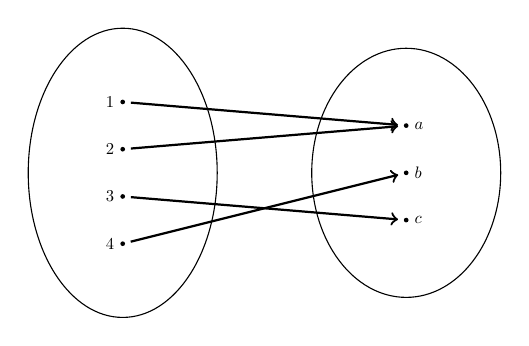
\begin{tikzpicture}[ele/.style={fill=black,circle,minimum width=.8pt,inner sep=1pt},every fit/.style={ellipse,draw,inner sep=35},scale=0.6, every node/.style={scale=0.6}]
    \node[ele,label=left:$1$] (a1) at (0,4) {};    
    \node[ele,label=left:$2$] (a2) at (0,3) {};    
    \node[ele,label=left:$3$] (a3) at (0,2) {};    
    \node[ele,label=left:$4$] (a4) at (0,1) {};
    
    \node[ele,label=right:$a$] (b1) at (6,3.5) {};
    \node[ele,label=right:$b$] (b2) at (6,2.5) {};
    \node[ele,label=right:$c$] (b3) at (6,1.5) {};
    
    \node[draw,fit= (a1) (a2) (a3) (a4),minimum width=4cm] {} ;
    \node[draw,fit= (b1) (b2) (b3),minimum width=4cm] {} ;  
    \draw[->,thick,shorten <=2pt,shorten >=2pt] (a1) -- (b1);
    \draw[->,thick,shorten <=2pt,shorten >=2] (a2) -- (b1);
    \draw[->,thick,shorten <=2pt,shorten >=2] (a3) -- (b3);
    \draw[->,thick,shorten <=2pt,shorten >=2] (a4) -- (b2);
\end{tikzpicture}
            \caption{A mapping that is not a bijection as two elements map to the same one.}
        \end{figure}
    }
    \addtocounter{figure}{1}
    \only<3>{%
        \begin{figure}
            \centering
            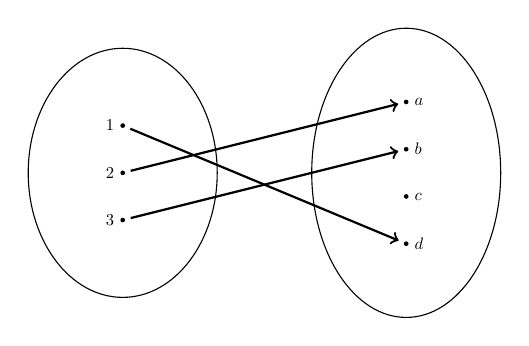
\begin{tikzpicture}[ele/.style={fill=black,circle,minimum width=.8pt,inner sep=1pt},every fit/.style={ellipse,draw,inner sep=35},scale=0.6, every node/.style={scale=0.6}]
    \node[ele,label=left:$1$] (a1) at (0,3.5) {};    
    \node[ele,label=left:$2$] (a2) at (0,2.5) {};    
    \node[ele,label=left:$3$] (a3) at (0,1.5) {};
    
    \node[ele,label=right:$a$] (b1) at (6,4) {};
    \node[ele,label=right:$b$] (b2) at (6,3) {};
    \node[ele,label=right:$c$] (b3) at (6,2) {};
    \node[ele,label=right:$d$] (b4) at (6,1) {};
    
    \node[draw,fit= (a1) (a2) (a3),minimum width=4cm] {} ;
    \node[draw,fit= (b1) (b2) (b3) (b4),minimum width=4cm] {} ;  
    \draw[->,thick,shorten <=2pt,shorten >=2pt] (a1) -- (b4);
    \draw[->,thick,shorten <=2pt,shorten >=2] (a2) -- (b1);
    \draw[->,thick,shorten <=2pt,shorten >=2] (a3) -- (b2);
\end{tikzpicture}
            \caption{A mapping that is not a bijection as there is an element in the codomain that no element maps to.}
        \end{figure}
    }
    \addtocounter{figure}{1}
    \onslide<4>{%
        \begin{figure}
            \centering
            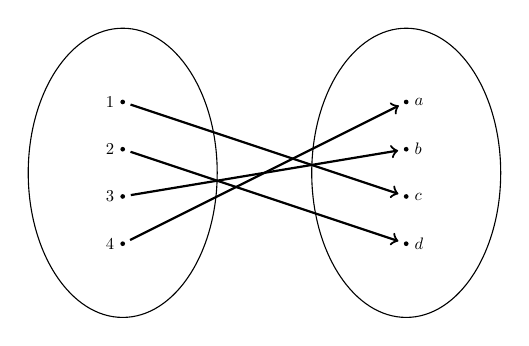
\begin{tikzpicture}[ele/.style={fill=black,circle,minimum width=.8pt,inner sep=1pt},every fit/.style={ellipse,draw,inner sep=35},scale=0.6, every node/.style={scale=0.6}]
    \node[ele,label=left:$1$] (a1) at (0,4) {};    
    \node[ele,label=left:$2$] (a2) at (0,3) {};    
    \node[ele,label=left:$3$] (a3) at (0,2) {};    
    \node[ele,label=left:$4$] (a4) at (0,1) {};
    
    \node[ele,label=right:$a$] (b1) at (6,4) {};
    \node[ele,label=right:$b$] (b2) at (6,3) {};
    \node[ele,label=right:$c$] (b3) at (6,2) {};
    \node[ele,label=right:$d$] (b4) at (6,1) {};
    
    \node[draw,fit= (a1) (a2) (a3) (a4),minimum width=4cm] {} ;
    \node[draw,fit= (b1) (b2) (b3) (b4),minimum width=4cm] {} ;  
    \draw[->,thick,shorten <=2pt,shorten >=2pt] (a1) -- (b3);
    \draw[->,thick,shorten <=2pt,shorten >=2] (a2) -- (b4);
    \draw[->,thick,shorten <=2pt,shorten >=2] (a3) -- (b2);
    \draw[->,thick,shorten <=2pt,shorten >=2] (a4) -- (b1);
\end{tikzpicture}
            \caption{A bijection.}
        \end{figure}
    }
\end{frame}
\begin{frame}{Size preserving bijections}
\begin{block}{Definition}<1->
A bijection $f$ between two combinatorial classes $\mathcal{C}$ and $\mathcal{D}$ is \emph{size preserving} if $|c| = |f(c)|$ for all $c\in\mathcal{C}$.
\end{block}
\begin{block}{Example}<2->
Flipping bits in binary strings.
\begin{align*}
    \begin{array}{ccc}
        0 & \mapsto & 1  \\
        0101 & \mapsto & 1010
    \end{array}
\end{align*}
\end{block}
\end{frame}
\begin{frame}{Counting sequence, generating function and isomorphism}
    \begin{definition}<1->
        The \emph{counting sequence} of a combinatorial class $\mathcal{C}$ is the infinite sequence
        \[
            |\mathcal{C}_0|, |\mathcal{C}_1|, |\mathcal{C}_2|, \dotsc
        \]
    \end{definition}
    \begin{definition}<2->
        Two classes, $\mathcal{C}$ and $\mathcal{D}$, with the same counting sequence are \emph{isomorphic}, $\mathcal{C} \cong \mathcal{D}$.
    \end{definition}
    \begin{definition}<3->
        The \emph{generating function} of a combinatorial class $\mathcal{C}$ is the power series
        \[
            \sum_{i=0}^\infty|\mathcal{C}_i|z^i.
        \]
    \end{definition}
\end{frame}
\begin{frame}{Symbolic method}
    The \emph{symbolic method} in \authcite{flajolet:ac} describes how combinatorial classes can be constructed. 
    \begin{itemize}
        \item \emph{Combinatorial specifications}
        \item \emph{Constructors}
        \item \emph{Atoms}
        \item \emph{Combinatorial rules}\footnote{Not a terminology from \authcite{flajolet:ac}}
    \end{itemize}
\end{frame}

{
\begin{frame}{Symbolic method - example}
    \begin{figure}
    \centering
    {
\newcommand{\rootcls}{(0\,|\,10)\!\ast(1\,|\,\varepsilon)}
\begin{tikzpicture}[remember picture,overlay,yshift=0cm,xshift=-1cm,scale=0.75, every node/.style={scale=0.7}]
    % slide 1
    \node (root) at (0, 0) {$\rootcls$};
    % slide 2
    \node<2-> (rootop) at (0,-1) {$\sqcup$};
    \draw<2-> (rootop) circle (0.2);
    \node<2-> (lvl11) at (-3,-2.5) {$0\rootcls$};
    \node<2-> (lvl12) at (0,-2.5) {$\varepsilon$};
    \node<2-> (lvl13) at (3,-2.5) {$1\,|\,(10\rootcls)$};
    \draw<2-> (root) -- (rootop);
    \draw<2-> \ptedge{(rootop)}{(-0.5,1.1)}{(lvl11)}{(-0.5,0.55)};
    \draw<2-> (rootop) -- (lvl12);
    \draw<2-> \ptedge{(rootop)}{(-0.5,1.1)}{(lvl13)}{(-0.5,0.55)};
    % slide 3 - rule
    \node<3-> [brownish,left=0.3cm of root] {$\mathcal{A}$};
    \node<3-> [brownish,left=0.3cm of lvl11] {$\mathcal{B}$};
    \node<3-> [brownish,right=0.3cm of lvl13] {$\mathcal{C}$};
    \draw<3-> [brownish,dotted] (-5.2,-8.3) rectangle (-2,-6.1);
    \draw<3-> [brownish,dotted] (-1.7,-8.3) rectangle (2.3,-6.1);
    \draw<3-> [brownish] (-5,-6.5) node[anchor=west] {$\mathcal{A} \cong \mathcal{B} \sqcup \set{\varepsilon}  \sqcup \mathcal{C}$};
    \draw<3-> [brownish] (-1.69,-6.5) node[anchor=west] {$A(z) = 1 + B(z) + C(z)$};
    % slide 4
    \node<4-> (lvl11op) at (-3,-3.5) {$\times$};
    \draw<4-> (lvl11op) circle (0.2);
    \node<4-> (lvl21) at (-5, -5) {$0$};
    \node<4-> (lvl22) at (-1, -5) {$\rootcls$};
    \draw<4-> (lvl11) -- (lvl11op);
    \draw<4-> \ptedge{(lvl11op)}{(-0.5,1.1)}{(lvl21)}{(-0.5,0.55)};
    \draw<4-> \ptedge{(lvl11op)}{(-0.5,1.1)}{(lvl22)}{(-0.5,0.55)};
    % slide 5 - rule
    \node<5-> [brownish,left=0.3cm of lvl22] {$\mathcal{A}$};
    \draw<5-> [brownish] (-4.96,-7) node[anchor=west] {$\mathcal{B} \cong \set{0} \times \mathcal{A}$};
    \draw<5-> [brownish] (-1.7,-7) node[anchor=west] {$B(z) = zA(z)$};
    % slide 6
    \node<6-> (lvl13op) at (3,-3.5) {$\sqcup$};
    \draw<6-> (lvl13op) circle (0.2);
    \node<6-> (lvl23) at (1, -5) {$1$};
    \node<6-> (lvl24) at (5, -5) {$10\rootcls$};
    \draw<6-> (lvl13) -- (lvl13op);
    \draw<6-> \ptedge{(lvl13op)}{(-0.5,1.1)}{(lvl23)}{(-0.5,0.55)};
    \draw<6-> \ptedge{(lvl13op)}{(-0.5,1.1)}{(lvl24)}{(-0.5,0.55)};
    % slide 7 - rule
    \node<7-> [brownish,right=0.3cm of lvl24] {$\mathcal{D}$};
    \draw<7-> [brownish] (-4.925,-7.5) node[anchor=west] {$\mathcal{C} \cong \set{1} \sqcup \mathcal{D}$};
    \draw<7-> [brownish] (-1.7,-7.5) node[anchor=west] {$C(z) = z + D(z)$};
    % slide 8 
    \node<8-> (lvl24op) at (5,-6) {$\times$};
    \draw<8-> (lvl24op) circle (0.2);
    \node<8-> (lvl31) at (3,-7.5) {$10$};
    \node<8-> (lvl32) at (7,-7.5) {$\rootcls$};
    \draw<8-> (lvl24) -- (lvl24op);
    \draw<8->\ptedge{(lvl24op)}{(-0.5,1.1)}{(lvl31)}{(-0.5,0.55)};
    \draw<8-> \ptedge{(lvl24op)}{(-0.5,1.1)}{(lvl32)}{(-0.5,0.55)};
    % slide 9 - rule
    \node<9-> [brownish,right=0.3cm of lvl32] {$\mathcal{A}$};
    \draw<9-> [brownish] (-5,-8) node[anchor=west] {$\mathcal{D} \cong \set{10} \times \mathcal{A}$};
    \draw<9-> [brownish] (-1.71,-8) node[anchor=west] {$D(z) = z^2A(z)$};
\end{tikzpicture}
}
    \end{figure}
    % Some horrible hack until I find out how to deal with overlay and captions...
    \onslide<9->{\begin{figure}\begin{tikzpicture}[yshift=-20cm]\draw[slideback,opacity=0] (0,0) -- (0,-6);\end{tikzpicture}\caption{A specification for binary strings avoiding repeated 1's.}\end{figure}}
\end{frame}

\begin{frame}{Symbolic method - example}
    \onslide<1->{%
    We now have a system of equations
    \[
    \systeme*{A(z) = 1 + B(z) + C(z), B(z) = zA(z), C(z) = z + D(z), D(z) = z^2A(z)}
    \]
    }
    \onslide<2->{%
    and solving for $A(z)$ gives
    \[
        A(z) = \frac{1+z}{1-z-z^2}.
    \]
    }
    \onslide<3->{%
    Taylor series at $z=0$ is
    \[
        A(z) = 1 + 2 z + 3 z^2 + 5 z^3 + 8 z^4 + 13 z^5 + 21 z^6 + 34 z^7 + 55 z^8 + \dotsm
    \]
    }
\end{frame}
}
\begin{frame}{Combinatorial Exploration}
    \begin{minipage}{0.5\textwidth}
    \begin{itemize}
        \item Combinatorial Exploration automates finding specifications
        \item Applies strategies in hope of creating rules
        \item Creates a universe of rules with a tree search
    \end{itemize}
    \end{minipage}
    \hfill
    \onslide<2>{%
    \begin{minipage}{0.45\textwidth}
    \begin{figure}
        \centering
        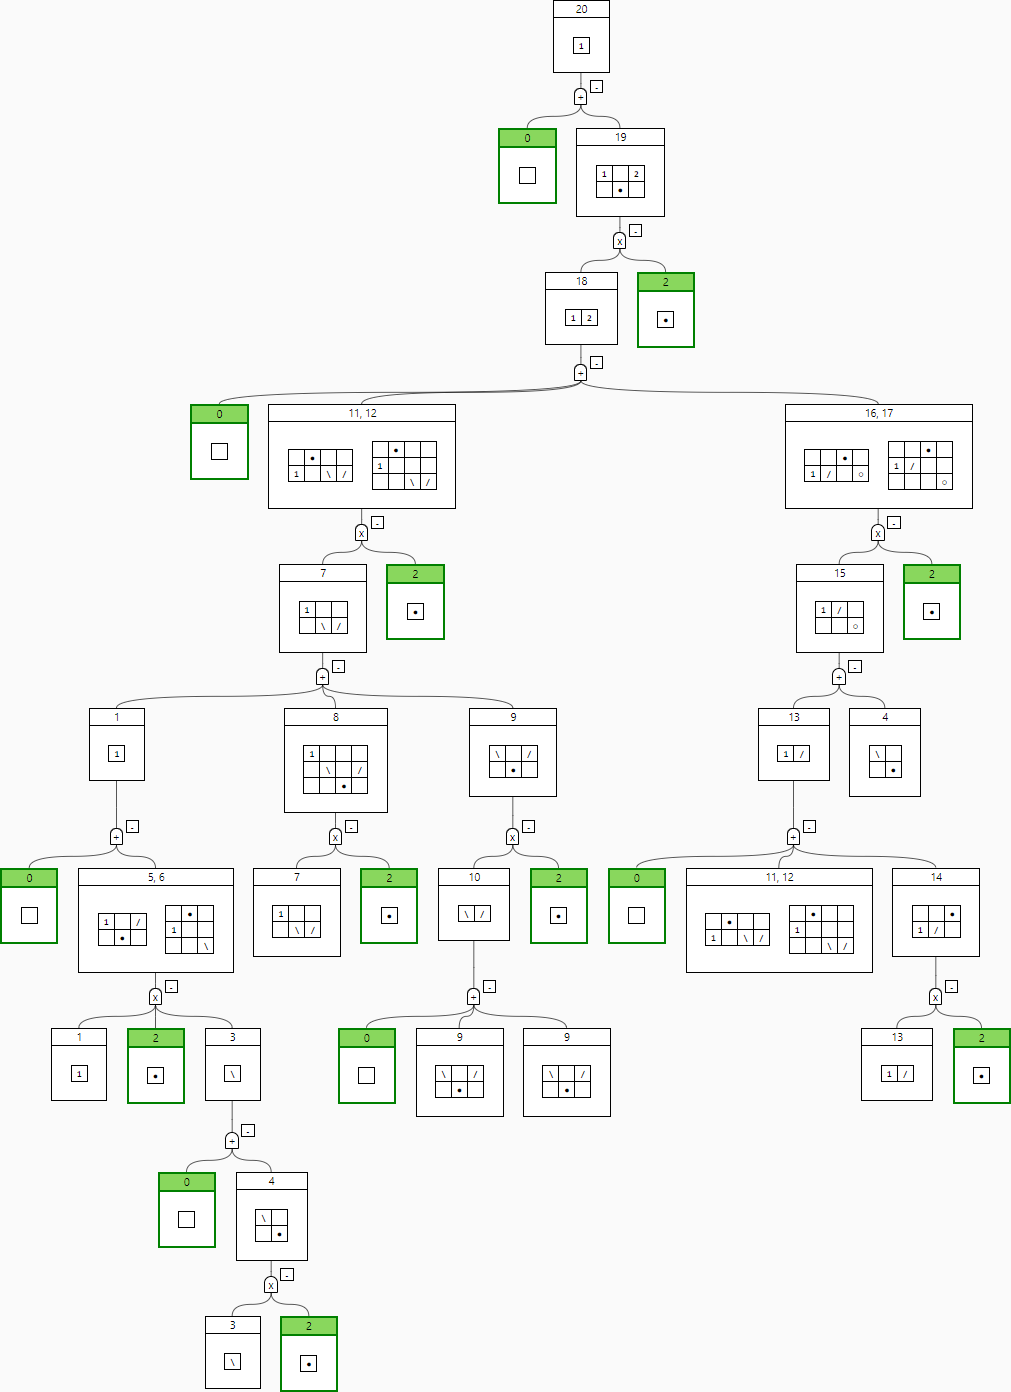
\includegraphics[scale=0.17]{graphics/cssoutput.png}
        \caption{Specification found by Combinatorial Exploration.}
    \end{figure}
    \end{minipage}
    }
\end{frame}
\begin{frame}{Permutation}
    \begin{block}{Definition}<1->
    A \emph{permutation} $\pi$ is a bijection between a set and itself.
    \end{block}
    \begin{block}{Example}<2->
        The permutations of size $3$ are
        \[
            123, 132, 213, 231, 312, 321.
        \]
    \end{block}
    \onslide<3->{%
    \begin{figure}
    \centering
    
    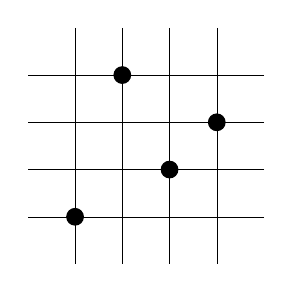
\begin{tikzpicture}[,scale=0.6, every node/.style={scale=0.6}]
            \foreach \x in {1,...,4} {
                    \draw[ultra thin] (\x,5)--(\x,0);
                    \draw[ultra thin] (5,\x)--(0,\x);
            }
            \draw[fill=black] (1,1) circle (5pt);
            \draw[fill=black] (2,4) circle (5pt);
            \draw[fill=black] (3,2) circle (5pt);
            \draw[fill=black] (4,3) circle (5pt);
    \end{tikzpicture}
    \caption{The graphical representation of $\pi=1423$.}
    \end{figure}
    }
\end{frame}
\begin{frame}{Permutation pattern}
    \begin{block}{Definition}<1->
    A permutation $\pi$ \emph{contains} another permutation $\sigma$ if a subsequence of $\pi$ has the same relative order as $\sigma$, denoted $\contains{\pi}{\sigma}$.
    \end{block}
    \begin{block}{Definition}<1->
    A permutation $\pi$ \emph{avoids} $\sigma$ if it does not contain it.
    \end{block}
    \only<2>{%
    \begin{figure}
        \centering
        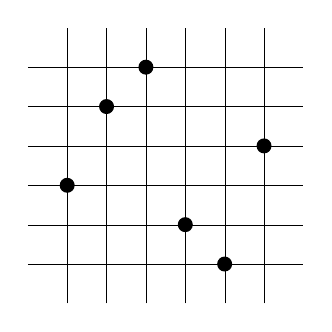
\begin{tikzpicture}[scale=.5,baseline=(current bounding box.center)]
\foreach \x in {1,...,6} {
    \draw[ultra thin] (\x,0)--(\x,7); %vline
    \draw[ultra thin] (0,\x)--(7,\x); %hline
}
\draw[fill=black] (1,3) circle (5pt);
\draw[fill=black] (2,5) circle (5pt);
\draw[fill=black] (3,6) circle (5pt);
\draw[fill=black] (4,2) circle (5pt);
\draw[fill=black] (5,1) circle (5pt);
\draw[fill=black] (6,4) circle (5pt);
\end{tikzpicture}
        \caption{The permutation $356214$.}
    \end{figure}
    }
    \addtocounter{figure}{1}
    \onslide<3->{%
    \begin{figure}
        \centering
        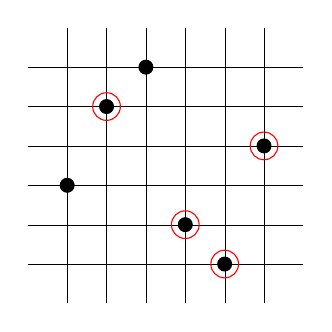
\begin{tikzpicture}[scale=.5,baseline=(current bounding box.center)]
\foreach \x in {1,...,6} {
    \draw[ultra thin] (\x,0)--(\x,7); %vline
    \draw[ultra thin] (0,\x)--(7,\x); %hline
}
\draw[fill=black] (1,3) circle (5pt);
\draw[fill=black] (2,5) circle (5pt);
\draw[fill=black] (3,6) circle (5pt);
\draw[fill=black] (4,2) circle (5pt);
\draw[fill=black] (5,1) circle (5pt);
\draw[fill=black] (6,4) circle (5pt);
\draw<3->[red] (2,5) circle (10pt);
\draw<3->[red] (4,2) circle (10pt);
\draw<3->[red] (5,1) circle (10pt);
\draw<3->[red] (6,4) circle (10pt);
\end{tikzpicture}
        \caption{An occurrence of $4213$ in $356214$.}
    \end{figure}
    }
\end{frame}
\begin{frame}{Permutation class}
    %\onslide<1->{%
    %Let $\mathcal{S}$ be the set of all permutations.
    %\[
        %\mathcal{S} = \set{\varepsilon, 1, 12, 21, 123, 132, 213, 231, 312, 321, \dotsc}
    %\]
    %}
    
    \onslide<1->{%
    A permutation $\pi$ avoids a set of permutations $\Pi$ if it avoids every $\sigma \in \Pi$.
    }
    
    \onslide<2->{%
    The set of permutations
    \[
        \Av{\Pi} = \cset{\pi}{\pi \text{ avoids } \Pi}
    \]
    is a \emph{permutation class}.
    }
\end{frame}
\begin{frame}{Cell}
    \begin{figure}
        \centering
        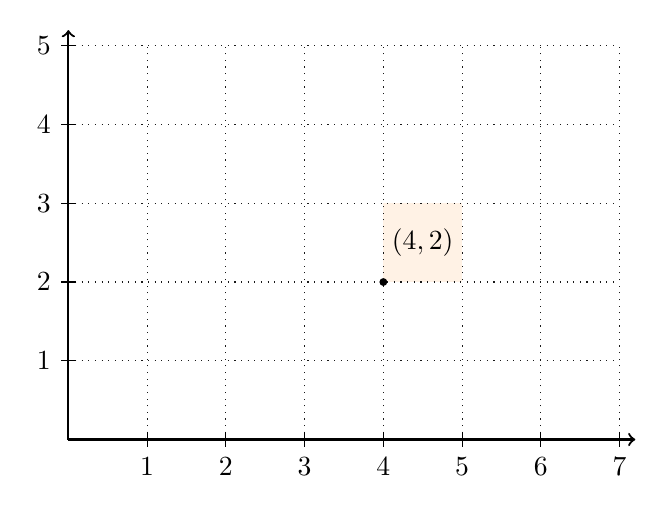
\begin{tikzpicture}
    \fill[orange!10] (4,2) rectangle (5,3);
    \draw[black!90,dotted] (0,0) grid (7,5);
    \draw[thick,->] (0,0) -- (7.2,0);
    \draw[thick,->] (0,0) -- (0,5.2);
    \foreach \x in {1,...,7} {%
        \draw (\x,.1) -- (\x,-.1) node[below] {$\x$};
    }
    \foreach \y in {1,...,5} {%
        \draw (.1,\y) -- (-.1,\y) node[left] {$\y$};
    }
    \fill (4,2) circle (0.05);
    \draw (4.5,2.5) node {$(4,2)$};
\end{tikzpicture}
        \caption{A cell $(c,r)\in\N^2$ defines the region $[c,c+1) \times [r,r+1)$.}
    \end{figure}
\end{frame}

\begin{frame}{Gridded permutation}
    \begin{block}{Definition\hfill(\authcite{albert2012geometric})}
    A pair $(\pi,P)$ where
    \begin{itemize}
        \item $\pi = \pi_1\pi_2 \dotsm \pi_n$ is a permutation
        \item $P = ((c_1,r_1),(c_2,r_2),\dotsc,(c_n,r_n))$ is a $n$-tuple of cells
    \end{itemize}
    is called a \emph{gridded permutation} \onslide<2->{if
    \begin{itemize}
        \item $i<j$ implies $c_i \leq c_j$
        \item $\pi_i < \pi_j$ implies $r_i \leq r_j$
    \end{itemize}
     for all $1 \leq i,j \leq n$.}
    \end{block}
\end{frame}

\begin{frame}{Gridded permutation - example}
\only<1>{\begin{figure}
    \centering
    \begin{tikzpicture}[scale=1.8]
    \draw[opacity=0] (0,0) rectangle (5,3);
    \end{tikzpicture}
    \caption{The gridded permutation with $\pi=87162435$ and $P=((0,2),(0,2),(1,0),(1,2),(1,0),(3,1),(3,0),(4,2))$.}
\end{figure}
\begin{frame}{Cell}
    \begin{figure}
        \centering
        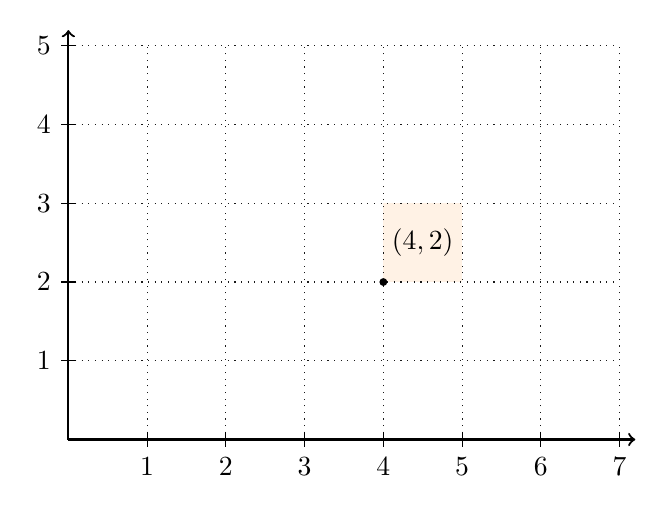
\begin{tikzpicture}
    \fill[orange!10] (4,2) rectangle (5,3);
    \draw[black!90,dotted] (0,0) grid (7,5);
    \draw[thick,->] (0,0) -- (7.2,0);
    \draw[thick,->] (0,0) -- (0,5.2);
    \foreach \x in {1,...,7} {%
        \draw (\x,.1) -- (\x,-.1) node[below] {$\x$};
    }
    \foreach \y in {1,...,5} {%
        \draw (.1,\y) -- (-.1,\y) node[left] {$\y$};
    }
    \fill (4,2) circle (0.05);
    \draw (4.5,2.5) node {$(4,2)$};
\end{tikzpicture}
        \caption{A cell $(c,r)\in\N^2$ defines the region $[c,c+1) \times [r,r+1)$.}
    \end{figure}
\end{frame}

\begin{frame}{Gridded permutation}
    \begin{block}{Definition\hfill(\authcite{albert2012geometric})}
    A pair $(\pi,P)$ where
    \begin{itemize}
        \item $\pi = \pi_1\pi_2 \dotsm \pi_n$ is a permutation
        \item $P = ((c_1,r_1),(c_2,r_2),\dotsc,(c_n,r_n))$ is a $n$-tuple of cells
    \end{itemize}
    is called a \emph{gridded permutation} \onslide<2->{if
    \begin{itemize}
        \item $i<j$ implies $c_i \leq c_j$
        \item $\pi_i < \pi_j$ implies $r_i \leq r_j$
    \end{itemize}
     for all $1 \leq i,j \leq n$.}
    \end{block}
\end{frame}

\begin{frame}{Gridded permutation - example}
\only<1>{\begin{figure}
    \centering
    \begin{tikzpicture}[scale=1.8]
    \draw[opacity=0] (0,0) rectangle (5,3);
    \end{tikzpicture}
    \caption{The gridded permutation with $\pi=87162435$ and $P=((0,2),(0,2),(1,0),(1,2),(1,0),(3,1),(3,0),(4,2))$.}
\end{figure}
\begin{frame}{Cell}
    \begin{figure}
        \centering
        \input{graphics/cell}
        \caption{A cell $(c,r)\in\N^2$ defines the region $[c,c+1) \times [r,r+1)$.}
    \end{figure}
\end{frame}

\begin{frame}{Gridded permutation}
    \begin{block}{Definition\hfill(\authcite{albert2012geometric})}
    A pair $(\pi,P)$ where
    \begin{itemize}
        \item $\pi = \pi_1\pi_2 \dotsm \pi_n$ is a permutation
        \item $P = ((c_1,r_1),(c_2,r_2),\dotsc,(c_n,r_n))$ is a $n$-tuple of cells
    \end{itemize}
    is called a \emph{gridded permutation} \onslide<2->{if
    \begin{itemize}
        \item $i<j$ implies $c_i \leq c_j$
        \item $\pi_i < \pi_j$ implies $r_i \leq r_j$
    \end{itemize}
     for all $1 \leq i,j \leq n$.}
    \end{block}
\end{frame}

\begin{frame}{Gridded permutation - example}
\only<1>{\begin{figure}
    \centering
    \begin{tikzpicture}[scale=1.8]
    \draw[opacity=0] (0,0) rectangle (5,3);
    \end{tikzpicture}
    \caption{The gridded permutation with $\pi=87162435$ and $P=((0,2),(0,2),(1,0),(1,2),(1,0),(3,1),(3,0),(4,2))$.}
\end{figure}
\input{graphics/gp}
}
\addtocounter{figure}{1}
\only<2>{\begin{figure}
    \centering
    \begin{tikzpicture}[scale=1.8]
    \draw[opacity=0] (0,0) rectangle (5,3);
    \end{tikzpicture}
    \caption{An occurrence of $3^{(0,2)}1^{(1,0)}2^{(3,1)}$ in the gridded permutation $87^{(0,2)}1^{(1,0)}6^{(1,2)}2^{(1,0)}4^{(3,1)}3^{(3,0)}5^{(4,2)}$.}
\end{figure}
\input{graphics/gppatt}
}
\end{frame}


%\begin{frame}{Gridded permutation - combinatorial class}
%    \begin{figure}
%        \centering
%        \input{graphics/gpclass}
%        \caption{The combinatorial class $\mathcal{G}^{(5,3)}$.}
%    \end{figure}
%\end{frame}
}
\addtocounter{figure}{1}
\only<2>{\begin{figure}
    \centering
    \begin{tikzpicture}[scale=1.8]
    \draw[opacity=0] (0,0) rectangle (5,3);
    \end{tikzpicture}
    \caption{An occurrence of $3^{(0,2)}1^{(1,0)}2^{(3,1)}$ in the gridded permutation $87^{(0,2)}1^{(1,0)}6^{(1,2)}2^{(1,0)}4^{(3,1)}3^{(3,0)}5^{(4,2)}$.}
\end{figure}
\begin{tikzpicture}[scale=1.8, every node/.style={scale=1.1},overlay,xshift=0.5cm,yshift=1.225cm]
  \def\xs{1.0}
  \def\ys{1.0}
  \def\ps{0.8}
  \draw (0.001,0.001) grid[xscale=\xs,yscale=\ys] (4.999, 2.999);
  \draw[rounded corners=2ex] (0,0) rectangle (5,3);
  \coordinate (p0) at (0.3333333333333333*\xs,2.8*\ys);
  \coordinate (p1) at (0.6666666666666666*\xs,2.6*\ys);
  \coordinate (p2) at (1.25*\xs,0.25*\ys);
  \coordinate (p3) at (1.5*\xs,2.4*\ys);
  \coordinate (p4) at (1.75*\xs,0.5*\ys);
  \coordinate (p5) at (3.3333333333333335*\xs,1.5*\ys);
  \coordinate (p6) at (3.6666666666666665*\xs,0.75*\ys);
  \coordinate (p7) at (4.5*\xs,2.2*\ys);
  \draw (p0)--(p1)--(p2)--(p3)--(p4)--(p5)--(p6)--(p7);
  \fill (p0) circle (0.1*\ps);
  \fill (p1) circle (0.1*\ps);
  \fill (p2) circle (0.1*\ps);
  \fill (p3) circle (0.1*\ps);
  \fill (p4) circle (0.1*\ps);
  \fill (p5) circle (0.1*\ps);
  \fill (p6) circle (0.1*\ps);
  \fill (p7) circle (0.1*\ps);
  \draw[red] (p1) circle (0.15*\ps);
  \draw[red] (p4) circle (0.15*\ps);
  \draw[red] (p5) circle (0.15*\ps);
\end{tikzpicture}
}
\end{frame}


%\begin{frame}{Gridded permutation - combinatorial class}
%    \begin{figure}
%        \centering
%        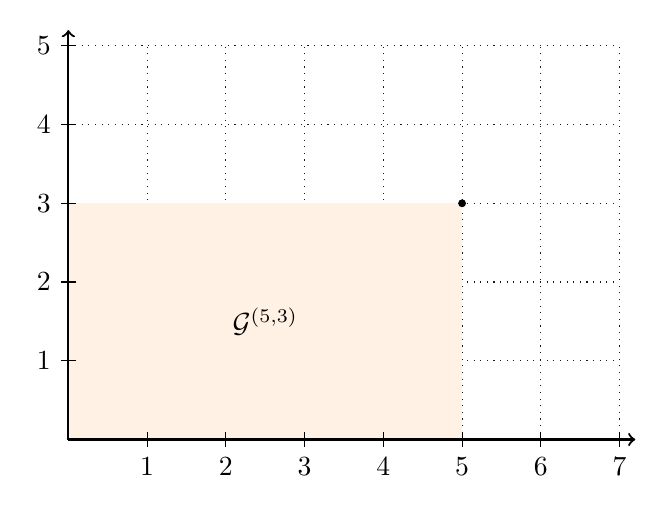
\begin{tikzpicture}
    \draw[black!90,dotted] (0,0) grid (7,5);
    \fill[orange!10] (0,0) rectangle (5,3);
    \draw[thick,->] (0,0) -- (7.2,0);
    \draw[thick,->] (0,0) -- (0,5.2);
    \foreach \x in {1,...,7} {%
        \draw (\x,.1) -- (\x,-.1) node[below] {$\x$};
    }
    \foreach \y in {1,...,5} {%
        \draw (.1,\y) -- (-.1,\y) node[left] {$\y$};
    }
    \fill (5,3) circle (0.05);
    \draw (2.5,1.5) node {$\mathcal{G}^{(5,3)}$};
\end{tikzpicture}
%        \caption{The combinatorial class $\mathcal{G}^{(5,3)}$.}
%    \end{figure}
%\end{frame}
}
\addtocounter{figure}{1}
\only<2>{\begin{figure}
    \centering
    \begin{tikzpicture}[scale=1.8]
    \draw[opacity=0] (0,0) rectangle (5,3);
    \end{tikzpicture}
    \caption{An occurrence of $3^{(0,2)}1^{(1,0)}2^{(3,1)}$ in the gridded permutation $87^{(0,2)}1^{(1,0)}6^{(1,2)}2^{(1,0)}4^{(3,1)}3^{(3,0)}5^{(4,2)}$.}
\end{figure}
\begin{tikzpicture}[scale=1.8, every node/.style={scale=1.1},overlay,xshift=0.5cm,yshift=1.225cm]
  \def\xs{1.0}
  \def\ys{1.0}
  \def\ps{0.8}
  \draw (0.001,0.001) grid[xscale=\xs,yscale=\ys] (4.999, 2.999);
  \draw[rounded corners=2ex] (0,0) rectangle (5,3);
  \coordinate (p0) at (0.3333333333333333*\xs,2.8*\ys);
  \coordinate (p1) at (0.6666666666666666*\xs,2.6*\ys);
  \coordinate (p2) at (1.25*\xs,0.25*\ys);
  \coordinate (p3) at (1.5*\xs,2.4*\ys);
  \coordinate (p4) at (1.75*\xs,0.5*\ys);
  \coordinate (p5) at (3.3333333333333335*\xs,1.5*\ys);
  \coordinate (p6) at (3.6666666666666665*\xs,0.75*\ys);
  \coordinate (p7) at (4.5*\xs,2.2*\ys);
  \draw (p0)--(p1)--(p2)--(p3)--(p4)--(p5)--(p6)--(p7);
  \fill (p0) circle (0.1*\ps);
  \fill (p1) circle (0.1*\ps);
  \fill (p2) circle (0.1*\ps);
  \fill (p3) circle (0.1*\ps);
  \fill (p4) circle (0.1*\ps);
  \fill (p5) circle (0.1*\ps);
  \fill (p6) circle (0.1*\ps);
  \fill (p7) circle (0.1*\ps);
  \draw[red] (p1) circle (0.15*\ps);
  \draw[red] (p4) circle (0.15*\ps);
  \draw[red] (p5) circle (0.15*\ps);
\end{tikzpicture}
}
\end{frame}


%\begin{frame}{Gridded permutation - combinatorial class}
%    \begin{figure}
%        \centering
%        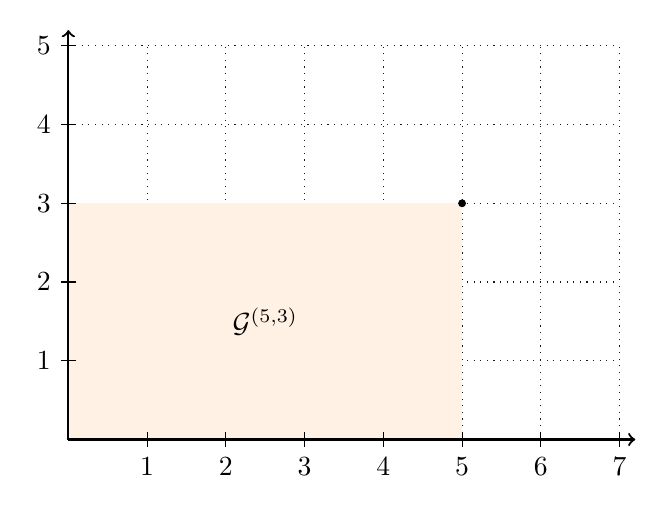
\begin{tikzpicture}
    \draw[black!90,dotted] (0,0) grid (7,5);
    \fill[orange!10] (0,0) rectangle (5,3);
    \draw[thick,->] (0,0) -- (7.2,0);
    \draw[thick,->] (0,0) -- (0,5.2);
    \foreach \x in {1,...,7} {%
        \draw (\x,.1) -- (\x,-.1) node[below] {$\x$};
    }
    \foreach \y in {1,...,5} {%
        \draw (.1,\y) -- (-.1,\y) node[left] {$\y$};
    }
    \fill (5,3) circle (0.05);
    \draw (2.5,1.5) node {$\mathcal{G}^{(5,3)}$};
\end{tikzpicture}
%        \caption{The combinatorial class $\mathcal{G}^{(5,3)}$.}
%    \end{figure}
%\end{frame}
\begin{frame}{Tiling}
    \begin{block}{Definition\hfill(\authcite{BeanPhd:phd})}
        A \emph{tiling} is a triple $\mathcal{T} = ((c,r), \mathcal{O}, \mathcal{R})$ where
        \begin{itemize}
            \item $(c,r) \in \Z^+ \times \Z^+$  is called \emph{dimension}
            \item $\mathcal{O} \subseteq \mathcal{G}^{(c,r)}$ is called \emph{obstructions}
            \item $\mathcal{R}=\set{\mathcal{R}_1,\mathcal{R}_2,\dotsc,\mathcal{R}_k} \subseteq \left(\mathcal{G}^{(c,r)}\right)^k$ is called \emph{requirements}
        \end{itemize}
    \end{block}
    \onslide<2->{The gridded permutations in $\textsf{Grid}(\mathcal{T})$ are those in $\mathcal{G}^{(c,r)}$ that 
    \begin{itemize}
        \item avoid $\mathcal{O}$
        \item contain $\mathcal{R}_1, \mathcal{R}_2, \dotsc, \mathcal{R}_k$
    \end{itemize}}
\end{frame}
\begin{frame}{Tiling - example}
    \begin{figure}
        \centering
        {
% rect
%\newcommand{\reqpnt}[3]{\fill[blue] (#1-#3,#2-#3) rectangle (#1+#3,#2+#3);}
% donut
%\newcommand{\reqpnt}[3]{\fill[blue] (#1,#2) circle (#3); \fill[white] (#1,#2) circle (#3 * 0.5);}
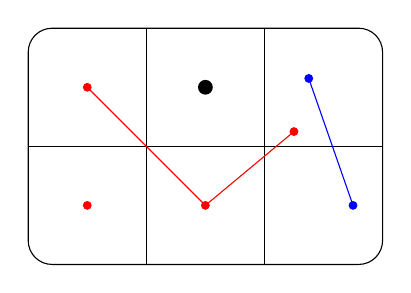
\begin{tikzpicture}[scale=0.75, every node/.style={scale=0.75}]
    \def\spnt{0.075} % Size of smaller points
    \def\lpnt{0.125} % Size of larger points
    \draw[rounded corners=2ex] (0,0) rectangle (6,4);
    \draw (2.0, 4) -- (2.0, 0);
    \draw (4.0, 4) -- (4.0, 0);
    \draw (0, 2) -- (6.0, 2);
    \fill[red] (1, 3) circle (\spnt);
    \fill[red] (1, 1) circle (\spnt);
    \fill[red] (3, 1) circle (\spnt);
    \fill[red] (4.5, 2.25) circle (\spnt);
    \draw[red] (1, 3) -- (3,1) -- (4.5,2.25);
    \fill (3,3) circle (\lpnt);
    \draw[blue] (4.75, 3.15) -- (5.5,1);
    \fill[blue] (4.75, 3.15) circle (\spnt);
    \fill[blue] (5.5, 1) circle (\spnt);
    %\reqpnt{4.75}{3.15}{\spnt*1.2}
    %\reqpnt{5.5}{1}{\spnt*1.2}
\end{tikzpicture}
}
        \caption{A tiling with $(c,r) = (3,2)$, $\mathcal{R} = \set{\set{1^{(1,1)}},\set{2^{(1,1)}1^{(2,0)}}}$ and $\mathcal{O} = \set{1^{(0,0)},12^{(1,1)},21^{(1,1)},3^{(0,1)}1^{(1,0)}2^{(2,1)}}$.}
    \end{figure}
\end{frame}

\section{Parallel Specifications}
%
\begin{frame}{Equivalent constructors}
    \begin{block}{Definition}
        Two constructors $\circ_1$ and $\circ_2$ are equivalent, $\circ_1 \equiv \circ_2$, if
        \[
            \sclsi{C}{1} \circ_1 \sclsi{C}{2} \circ_1 \dotsm \circ_1 \sclsi{C}{n} \cong \sclsi{D}{1} \circ_2 \sclsi{D}{2} \circ_2 \dotsm \circ_2 \sclsi{D}{n}
        \]
        for all classes $\sclsi{C}{1},\sclsi{C}{2},\dotsc,\sclsi{C}{n}$ and $\sclsi{D}{1},\sclsi{D}{2},\dotsc,\sclsi{D}{n}$ in the domain of $\circ_1$ and $\circ_2$ respectively where there exists a $\pi\in\mathcal{S}_n$ such that $\sclsi{C}{i}\cong\sclsi{D}{\pi_i}$ for all $i\in[n]$.
    \end{block}
\end{frame}
\begin{frame}{Parallel specifications}
    \begin{block}{Definition}
        Two specifications $\spec{C}$ and $\spec{D}$ are \emph{parallel} if the empty rooted paths in their respective specification graphs are matchable.
    \end{block}
    \onslide<2->{
    Two specifications are parallel if (recursively from the root) every class pair $\mathcal{C}$ and $\mathcal{D}$
    \begin{itemize}
        \item Both contain a single object which are equal in size.
        \item There is a recursion at an equal distance to an ancestor for both.
        \item Their constructors are equivalent and there is a bijection between their children such that we can match them this way.
    \end{itemize}
    Special attention to equivalence rules, $\mathcal{C}^{(1)} \cong \mathcal{C}^{(2)}$.
    }
\end{frame}
\begin{frame}{Parallel specifications - example}
    \begin{figure}
        \centering
        \begin{tikzpicture}
        \useasboundingbox (0,0) rectangle (10,7.5);
        %\draw [blue!30,dotted] (current bounding box.north west) rectangle (current bounding box.south east);
        \draw [black,opacity=0] (5,0) -- (5,7.5);
        \end{tikzpicture}
        \caption{Two parallel specifications.}
    \end{figure}
    \begin{tikzpicture}[remember picture,overlay]
        \node[at=(current page.center),yshift=-0.2cm,xshift=-(\paperwidth+1cm)*0.26]{{

\newcommand{\tone}{%
\begin{tikzpicture}[scale=0.25, every node/.style={scale=0.25}, baseline=(current bounding box.center)]
\def\xscale{1} % Horizontal scale factor
\def\yscale{1} % Vertical scale factor
\def\spnt{0.15} % Size of smaller points
\def\lpnt{0.125} % Size of larger points
\draw (3.52*\xscale, 3.76*\yscale) -- (3.52*\xscale, 0);
\useasboundingbox (0,0) rectangle (7.04*\xscale,3.76*\yscale);
\draw[rounded corners=2ex*0.25] (0,0) rectangle (7.04*\xscale,3.76*\yscale);
\fill[red] (4.55*\xscale, 1.18*\yscale) circle (\spnt);
\fill[red] (6.05*\xscale, 2.78*\yscale) circle (\spnt);
\draw[red] (4.55*\xscale, 1.18*\yscale) -- (6.05*\xscale,2.78*\yscale);
\fill[red] (4.55*\xscale, 2.79*\yscale) circle (\spnt);
\fill[red] (6.05*\xscale, 1.12*\yscale) circle (\spnt);
\draw[red] (4.55*\xscale, 2.79*\yscale) -- (6.05*\xscale,1.12*\yscale);
\fill[red] (2.67*\xscale, 3.21*\yscale) circle (\spnt);
\fill[red] (4.29*\xscale, 0.3*\yscale) circle (\spnt);
\draw[red] (2.67*\xscale, 3.21*\yscale) -- (4.29*\xscale,0.3*\yscale);
\fill[red] (1.09*\xscale, 3.07*\yscale) circle (\spnt);
\fill[red] (1.526001050877835*\xscale, 3.393088634545991*\yscale) circle (\spnt);
\fill[red] (2.13*\xscale, 2.55*\yscale) circle (\spnt);
\draw[red] (1.09*\xscale, 3.07*\yscale) -- (1.526001050877835*\xscale,3.393088634545991*\yscale) -- (2.13*\xscale,2.55*\yscale);
\fill[red] (0.64*\xscale, 1.39*\yscale) circle (\spnt);
\fill[red] (1.01*\xscale, 0.79*\yscale) circle (\spnt);
\fill[red] (1.35*\xscale, 1.03*\yscale) circle (\spnt);
\draw[red] (0.64*\xscale, 1.39*\yscale) -- (1.01*\xscale,0.79*\yscale) -- (1.35*\xscale,1.03*\yscale);
\fill[red] (1.98*\xscale, 1.84*\yscale) circle (\spnt);
\fill[red] (2.3511520552717013*\xscale, 1.3932029657051672*\yscale) circle (\spnt);
\fill[red] (2.71*\xscale, 0.92*\yscale) circle (\spnt);
\draw[red] (1.98*\xscale, 1.84*\yscale) -- (2.3511520552717013*\xscale,1.3932029657051672*\yscale) -- (2.71*\xscale,0.92*\yscale);
\end{tikzpicture} 
}

\newcommand{\ttwo}{%
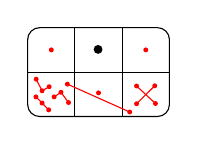
\begin{tikzpicture}[scale=0.3, every node/.style={scale=0.3}, baseline=(current bounding box.center)]
\def\xscale{1.0} % Horizontal scale factor
\def\yscale{1.0} % Vertical scale factor
\def\spnt{0.075*1.4} % Size of smaller points
\def\lpnt{0.125*1.5} % Size of larger points
\useasboundingbox (0,0) rectangle (6*\xscale,3.76*\yscale);
\draw[rounded corners=2ex*0.5] (0,0) rectangle (6*\xscale,3.76*\yscale);
\draw (2.0*\xscale, 3.76*\yscale) -- (2.0*\xscale, 0);
\draw (4.0*\xscale, 3.76*\yscale) -- (4.0*\xscale, 0);
\draw (0, 1.88*\yscale) -- (6.0*\xscale, 1.88*\yscale);
\fill[red] (4.61*\xscale, 0.54*\yscale) circle (\spnt);
\fill[red] (5.38*\xscale, 1.3*\yscale) circle (\spnt);
\draw[red] (4.61*\xscale, 0.54*\yscale) -- (5.38*\xscale,1.3*\yscale);
\fill[red] (1.68*\xscale, 1.37*\yscale) circle (\spnt);
\fill[red] (4.32*\xscale, 0.19*\yscale) circle (\spnt);
\draw[red] (1.68*\xscale, 1.37*\yscale) -- (4.32*\xscale,0.19*\yscale);
\fill[red] (4.61*\xscale, 1.29*\yscale) circle (\spnt);
\fill[red] (5.41*\xscale, 0.55*\yscale) circle (\spnt);
\draw[red] (4.61*\xscale, 1.29*\yscale) -- (5.41*\xscale,0.55*\yscale);
\fill[red] (1.12*\xscale, 0.83*\yscale) circle (\spnt);
\fill[red] (1.4096601986560762*\xscale, 1.0249991174784614*\yscale) circle (\spnt);
\fill[red] (1.73*\xscale, 0.59*\yscale) circle (\spnt);
\draw[red] (1.12*\xscale, 0.83*\yscale) -- (1.4096601986560762*\xscale,1.0249991174784614*\yscale) -- (1.73*\xscale,0.59*\yscale);
\fill[red] (1*\xscale, 2.82*\yscale) circle (\spnt);
\fill[red] (5*\xscale, 2.82*\yscale) circle (\spnt);
\fill[red] (3*\xscale, 1*\yscale) circle (\spnt);
\fill[red] (0.36*\xscale, 1.58*\yscale) circle (\spnt);
\fill[red] (0.6091281492290661*\xscale, 1.0877096738635244*\yscale) circle (\spnt);
\fill[red] (0.91*\xscale, 1.26*\yscale) circle (\spnt);
\draw[red] (0.36*\xscale, 1.58*\yscale) -- (0.6091281492290661*\xscale,1.0877096738635244*\yscale) -- (0.91*\xscale,1.26*\yscale);
\fill[red] (0.35*\xscale, 0.83*\yscale) circle (\spnt);
\fill[red] (0.61*\xscale, 0.57*\yscale) circle (\spnt);
\fill[red] (0.89*\xscale, 0.28*\yscale) circle (\spnt);
\draw[red] (0.35*\xscale, 0.83*\yscale) -- (0.61*\xscale,0.57*\yscale) -- (0.89*\xscale,0.28*\yscale);
\fill (2.98*\xscale,2.84*\yscale) circle (\lpnt);
\end{tikzpicture}
}

\newcommand{\tthree}{%
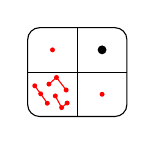
\begin{tikzpicture}[scale=0.3, every node/.style={scale=0.3}, baseline=(current bounding box.center)]
\def\xscale{1.0} % Horizontal scale factor
\def\yscale{1.0} % Vertical scale factor
\def\spnt{0.075*1.4} % Size of smaller points
\def\lpnt{0.125*1.5} % Size of larger points
\useasboundingbox (0,0) rectangle (4.2*\xscale,3.76*\yscale);
\draw[rounded corners=2ex*0.5] (0,0) rectangle (4.2*\xscale,3.76*\yscale);
\draw (2.1*\xscale, 3.76*\yscale) -- (2.1*\xscale, 0);
\draw (0, 1.88*\yscale) -- (4.2*\xscale, 1.88*\yscale);
\fill[red] (1.05*\xscale, 2.82*\yscale) circle (\spnt);
\fill[red] (3.15*\xscale, 0.94*\yscale) circle (\spnt);
\fill[red] (0.9*\xscale, 1.37*\yscale) circle (\spnt);
\fill[red] (1.2199471753311761*\xscale, 1.6524363073940609*\yscale) circle (\spnt);
\fill[red] (1.63*\xscale, 1.12*\yscale) circle (\spnt);
\draw[red] (0.9*\xscale, 1.37*\yscale) -- (1.2199471753311761*\xscale,1.6524363073940609*\yscale) -- (1.63*\xscale,1.12*\yscale);
\fill[red] (1.17*\xscale, 0.87*\yscale) circle (\spnt);
\fill[red] (1.436829177631258*\xscale, 0.37686266458866924*\yscale) circle (\spnt);
\fill[red] (1.67*\xscale, 0.57*\yscale) circle (\spnt);
\draw[red] (1.17*\xscale, 0.87*\yscale) -- (1.436829177631258*\xscale,0.37686266458866924*\yscale) -- (1.67*\xscale,0.57*\yscale);
\fill[red] (0.3*\xscale, 1.3*\yscale) circle (\spnt);
\fill[red] (0.55*\xscale, 0.96*\yscale) circle (\spnt);
\fill[red] (0.83*\xscale, 0.56*\yscale) circle (\spnt);
\draw[red] (0.3*\xscale, 1.3*\yscale) -- (0.55*\xscale,0.96*\yscale) -- (0.83*\xscale,0.56*\yscale);
\fill (3.150000000000005*\xscale,2.8210223642172525*\yscale) circle (\lpnt);
\end{tikzpicture}
}

\newcommand{\tfour}{%
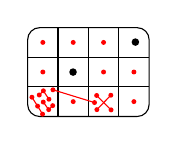
\begin{tikzpicture}[scale=0.3, every node/.style={scale=0.3}, baseline=(current bounding box.center)]
\def\xscale{1.0} % Horizontal scale factor
\def\yscale{1.0} % Vertical scale factor
\def\spnt{0.075*1.4} % Size of smaller points
\def\lpnt{0.16} % Size of larger points
\useasboundingbox (0,0) rectangle (5.14*\xscale,3.76*\yscale);
\draw[rounded corners=2ex*0.5] (0,0) rectangle (5.14*\xscale,3.76*\yscale);
\draw (1.285*\xscale, 3.76*\yscale) -- (1.285*\xscale, 0);
\draw (2.57*\xscale, 3.76*\yscale) -- (2.57*\xscale, 0);
\draw (3.855*\xscale, 3.76*\yscale) -- (3.855*\xscale, 0);
\draw (0, 1.2533333333333332*\yscale) -- (5.14*\xscale, 1.2533333333333332*\yscale);
\draw (0, 2.5066666666666664*\yscale) -- (5.14*\xscale, 2.5066666666666664*\yscale);
\fill[red] ({(0*1.285+0.6425)*\xscale}, {(1*1.253+0.63)*\yscale}) circle (\spnt);
\fill[red] ({(0*1.285+0.6425)*\xscale}, {(2*1.253+0.63)*\yscale}) circle (\spnt);
\fill[red] ({(1*1.285+0.6425)*\xscale}, {(0*1.253+0.63)*\yscale}) circle (\spnt);
\fill[red] ({(1*1.285+0.6425)*\xscale}, {(2*1.253+0.63)*\yscale}) circle (\spnt);
\fill[red] ({(2*1.285+0.6425)*\xscale}, {(1*1.253+0.63)*\yscale}) circle (\spnt);
\fill[red] ({(2*1.285+0.6425)*\xscale}, {(2*1.253+0.63)*\yscale}) circle (\spnt);
\fill[red] ({(3*1.285+0.6425)*\xscale}, {(0*1.253+0.63)*\yscale}) circle (\spnt);
\fill[red] ({(3*1.285+0.6425)*\xscale}, {(1*1.253+0.63)*\yscale}) circle (\spnt);
\fill[red] (2.93*\xscale, 0.29*\yscale) circle (\spnt);
\fill[red] (3.52*\xscale, 0.9*\yscale) circle (\spnt);
\draw[red] (2.93*\xscale, 0.29*\yscale) -- (3.52*\xscale,0.9*\yscale);
\fill[red] (1.07*\xscale, 1.13*\yscale) circle (\spnt);
\fill[red] (2.83*\xscale, 0.59*\yscale) circle (\spnt);
\draw[red] (1.07*\xscale, 1.13*\yscale) -- (2.83*\xscale,0.59*\yscale);
\fill[red] (2.92*\xscale, 0.89*\yscale) circle (\spnt);
\fill[red] (3.53*\xscale, 0.28*\yscale) circle (\spnt);
\draw[red] (2.92*\xscale, 0.89*\yscale) -- (3.53*\xscale,0.28*\yscale);
\fill[red] (0.49*\xscale, 0.91*\yscale) circle (\spnt);
\fill[red] (0.6644210751853692*\xscale, 1.086774200246225*\yscale) circle (\spnt);
\fill[red] (0.9*\xscale, 0.73*\yscale) circle (\spnt);
\draw[red] (0.49*\xscale, 0.91*\yscale) -- (0.6644210751853692*\xscale,1.086774200246225*\yscale) -- (0.9*\xscale,0.73*\yscale);
\fill[red] (0.66*\xscale, 0.61*\yscale) circle (\spnt);
\fill[red] (0.89*\xscale, 0.29*\yscale) circle (\spnt);
\fill[red] (1.06*\xscale, 0.46*\yscale) circle (\spnt);
\draw[red] (0.66*\xscale, 0.61*\yscale) -- (0.89*\xscale,0.29*\yscale) -- (1.06*\xscale,0.46*\yscale);
\fill[red] (0.18033887520734232*\xscale, 0.816133743581277*\yscale) circle (\spnt);
\fill[red] (0.42*\xscale, 0.44*\yscale) circle (\spnt);
\fill[red] (0.63*\xscale, 0.1*\yscale) circle (\spnt);
\draw[red] (0.18033887520734232*\xscale, 0.816133743581277*\yscale) -- (0.42*\xscale,0.44*\yscale) -- (0.63*\xscale,0.1*\yscale);
\fill (1.92*\xscale,1.88*\yscale) circle (\lpnt);
\fill (4.56*\xscale,3.15*\yscale) circle (\lpnt);
\end{tikzpicture}
}

\newcommand{\tpair}{%
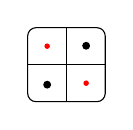
\begin{tikzpicture}[scale=0.25, every node/.style={scale=0.25}, baseline=(current bounding box.center)]
\def\xscale{1.0} % Horizontal scale factor
\def\yscale{1.0} % Vertical scale factor
\def\spnt{0.14} % Size of smaller points
\def\lpnt{0.2} % Size of larger points
\useasboundingbox (0,0) rectangle (3.94*\xscale,3.76*\yscale);
\draw[rounded corners=2ex*.35] (0,0) rectangle (3.94*\xscale,3.76*\yscale);
\draw (1.97*\xscale, 3.76*\yscale) -- (1.97*\xscale, 0);
\draw (0, 1.88*\yscale) -- (3.94*\xscale, 1.88*\yscale);
\fill (0.99*\xscale,0.864920127795527*\yscale) circle (\lpnt);
\fill (2.97*\xscale,2.841054313099042*\yscale) circle (\lpnt);
\fill[red] (0.99*\xscale,3.76*0.75*\yscale) circle (\spnt);
\fill[red] (3*0.99*\xscale,3.76*0.25*\yscale) circle (\spnt);
\end{tikzpicture}
}

\newcommand{\pntatom}{\tikz\fill (0,0) circle (0.1);}


\begin{tikzpicture}
    \draw [black,opacity=0] (-3.25,-6.87) rectangle (2.75,0.60);
    %\viewborder
    
    \node (rootB) at (0, 0) {\tone};
    
    \node<1,3-> (lvl11B) at (-1.5,-1.75) {\ttwo};
    \node<1,3-6,12-> (lvl12B) at (0,-1.75) {$\varepsilon$};
    \node<1,3-6,13-> (lvl13B) at (1.5,-1.75) {\tthree};
    \draw<1,3->\ptedge{(rootB.south)}{(-0.5,1.4)}{(lvl11B)}{(-0.5,0.9)};
    \draw<1,3-6,12->\ptedge{(rootB.south)}{(-0.5,1.4)}{(lvl12B)}{(-0.5,0.5)};
    \draw<1,3-6,13->\ptedge{(rootB.south)}{(-0.5,1.4)}{(lvl13B)}{(-0.5,0.9)};
    \circover{0,-.725}{0.13}{\tiny $\sqcup$}{1,3-}
    
    % Bijection greens and eq examples
    \draw<4>[orange] (lvl11B.south west) rectangle (lvl13B.north east);
    \draw<5> (-1.5, -3.5) node {$\mathcal{A}$};
    \draw<5> (lvl11B.south) -- (-1.5,-3.25);
    \draw<5> (-1.5, -5) node {$\mathcal{B}$};
    \draw<5> (-1.5,-3.75) -- (-1.5,-4.75);
    \draw<5> (1.5, -3.5) node {$\mathcal{C}$};
    \draw<5> (lvl13B.south) -- (1.5,-3.25);
    \draw<5> [orange] (-1.5-0.25,-5-0.25) rectangle (-1.5+.25,-5+.25);
    \draw<5> [orange] (1.5-0.25,-3.5-0.25) rectangle (1.5+.25,-3.5+.25);
    \draw<5> [orange] (0-.25,-1.75-.2) rectangle (0+.25,-1.75+.2);
    \circover{-1.5,-2.65}{0.13}{\tiny $\cong$}{5}
    \circover{-1.5,-3.95}{0.13}{\tiny $\cong$}{5}
    \circover{1.5,-2.65}{0.13}{\tiny $\cong$}{5}
    
    \node<1,7-> (lvl21B) at (-2.25,-3.5) {\tone};
    \coordinate (lvl22Bphantom) at (-0.75,-3.15);
    \node<1,7-> (lvl22B) at (-0.75,-3.5) {\pntatom};
    \draw<1,7->\ptedge{(lvl11B.south)}{(-0.5,1.4)}{(lvl21B)}{(-0.5,0.8)};
    \draw<1,7->\ptedge{(lvl11B.south)}{(-0.5,1.4)}{(lvl22Bphantom)}{(-0.5,0.45)};
    \draw<1,7-> ([yshift=0.18cm]lvl22Bphantom) -- (lvl22B);
    \circover{-1.5,-2.6}{0.13}{\tiny $\times$}{1,7-}
    
    \node<1,13-> (lvl23B) at (0.75,-3.5) {\tfour};
    \coordinate (lvl24Bphantom) at (2.25,-3.05);
    \node<1,13-> (lvl24B) at (2.25,-3.5) {\pntatom};
    \draw<1,13->\ptedge{(lvl13B.south)}{(-0.5,1.4)}{(lvl23B)}{(-0.5,0.89)};
    \draw<1,13->\ptedge{(lvl13B.south)}{(-0.5,1.4)}{(lvl24Bphantom)}{(-0.5,0.45)};
    \draw<1,13-> ([yshift=0.145cm]lvl24Bphantom) -- (lvl24B);
    \circover{1.5,-2.6}{0.13}{\tiny $\sqcup$}{1,13-}
    
    \node<1,14-> (lvl31B) at (0.75-1,-5.25) {\tpair};
    \node<1,14-> (lvl32B) at (0.75+1,-5.25) {\tone};
    \draw<1,14->\ptedge{(lvl23B.south)}{(-0.5,1.4)}{(lvl31B)}{(-0.5,0.8)};
    \draw<1,14->\ptedge{(lvl23B.south)}{(-0.5,1.4)}{(lvl32B)}{(-0.5,0.8)};
    \circover{0.75,-4.34}{0.13}{\tiny $\times$}{1,14-}
    
    \node<1,15-> (lvl41B) at (-1.25,-7+.35) {\pntatom};
    \node<1,15-> (lvl42B) at (0.75,-7+.35) {\pntatom};
    \draw<1,15->\ptedge{(lvl31B.south)}{(-0.5,1.4)}{(lvl41B)}{(-0.5,0.475)};
    \draw<1,15->\ptedge{(lvl31B.south)}{(-0.5,1.4)}{(lvl42B)}{(-0.5,0.475)};
    \circover{-.25,-6}{0.13}{\tiny $\times$}{1,15-}
\end{tikzpicture}
}};
    \end{tikzpicture}
    \begin{tikzpicture}[remember picture,overlay]
        \node[at=(current page.center),yshift=-0.2cm,xshift=(\paperwidth-1cm)*0.26]{{

\newcommand{\binroot}{(0\,|\,10)\!\ast(1\,|\,\varepsilon)}

\newcommand{\binsize}{\fontsize{7pt}{7pt}}

\begin{tikzpicture}
    \draw [black,opacity=0]  (-3.2,-6.87) rectangle (2.8,0.60);
    %\viewborder
    
    \node (rootA) at (0,0) {\binsize$\binroot$};
    
    \node<1,3-7,13-> (lvl11A) at (-1.75,-1.75) {\binsize$1|(01\binroot)$};
    \node<1,3-6,8,12-> (lvl12A) at (0,-1.75) {\binsize$\varepsilon$};
    \node<1,3-6,9-> (lvl13A) at (1.25,-1.75) {\binsize$0\binroot$};
    \draw<1,3-7,13->\ptedge{(rootA.south)}{(-0.5,1.4)}{(lvl11A)}{(0,0.55)};
    \draw<1,3-6,8,12->\ptedge{(rootA.south)}{(-0.5,1.4)}{(lvl12A)}{(-0.5,0.55)};
    \draw<1,3-6,9->\ptedge{(rootA.south)}{(-0.5,1.4)}{(lvl13A)}{(-0.5,0.55)};
    \circover{0,-0.4}{0.13}{\tiny $\sqcup$}{1,3-}
    
    \draw<4>[orange] (lvl11A.south west) rectangle (lvl13A.north east);
    
    \draw<5> (-1.75, -3.5) node {$\mathcal{D}$};
    \draw<5> (lvl11A.south) -- (-1.75,-3.25);
    \circover{-1.75,-2.2}{0.13}{\tiny $\cong$}{5}
    \draw<5> [orange] (-1.75-0.25,-3.5-0.25) rectangle (-1.75+.25,-3.5+.25);
    \draw<5>[orange] ([yshift=-0.05cm,xshift=-.05cm]lvl12A.south west) rectangle (lvl13A.north east);
    
    \node<1,7,13-> (lvl21A) at (-1.75-0.75,-3.5) {\binsize$1$};
    \node<1,7,13-> (lvl22A) at (-1.75+0.75,-3.5) {\binsize$10\binroot$};
    \draw<1,7,13->\ptedge{(lvl11A.south)}{(-0.5,1.4)}{(lvl21A)}{(-0.5,0.55)};
    \draw<1,7,13->\ptedge{(lvl11A.south)}{(-0.5,1.4)}{(lvl22A)}{(-0.5,0.55)};
    \circover{-1.75,-2.15}{0.13}{\tiny $\sqcup$}{1,7,13-}
    
    \node<1,9-> (lvl23A) at (1.25-0.6,-3.5) {\binsize$0$};
    \node<1,9,11-> (lvl24A) at (1.25+0.6,-3.5) {\binsize$\binroot$};
    \draw<10> (1.25+0.6,-3.5) node {$\mathcal{A}$};
    \draw<10>[-] (1.25+0.6,-3.8) -- (1.25+0.6,-4.8);
    \circover{1.25+0.6,-4.05}{0.13}{\tiny $\cong$}{10}
    \draw<10> (1.25+0.6,-5) node {\binsize$\binroot$};
    
    \draw<1,9->\ptedge{(lvl13A.south)}{(-0.5,1.4)}{(lvl23A)}{(-0.5,0.55)};
    \draw<1,9->\ptedge{(lvl13A.south)}{(-0.5,1.4)}{(lvl24A)}{(-0.5,0.55)};
    \circover{1.25,-2.15}{0.13}{\tiny $\times$}{1,9-}
    
    \node<1,14-> (lvl31A) at (-1.75+0.75-1,-5.25) {\binsize$10$};
    \node<1,14-> (lvl32A) at (-1.75+0.75+1,-5.25) {\binsize$\binroot$};
    \draw<1,14->\ptedge{(lvl22A.south)}{(-0.5,1.4)}{(lvl31A)}{(-0.5,0.55)};
    \draw<1,14->\ptedge{(lvl22A.south)}{(-0.5,1.4)}{(lvl32A)}{(-0.5,0.55)};
    \circover{-1,-3.9}{0.13}{\tiny $\times$}{1,14-}
    
    \node<1,15-> (lvl41A) at (-1.75+0.75-1-.95,-7+.35) {\binsize$1$};
    \node<1,15-> (lvl42A) at (-1.75+0.75-1+.95,-7+.35) {\binsize$0$};
    \draw<1,15->\ptedge{(lvl31A.south)}{(-0.5,1.4)}{(lvl41A)}{(-0.5,0.55)};
    \draw<1,15->\ptedge{(lvl31A.south)}{(-0.5,1.4)}{(lvl42A)}{(-0.5,0.55)};
    \circover{-2,-5.625}{0.13}{\tiny $\times$}{1,15-}
\end{tikzpicture}
}};
    \end{tikzpicture}
\end{frame}

\section{Parallel Bijections}

\begin{frame}{Parallel bijection}
    \begin{definition}
    If $\spec{C}$ and $\spec{D}$ are two parallel specifications with path matching $\gamma_{\spec{C},\spec{D}}$ and root classes $\mathcal{C}$ and $\mathcal{D}$, then their \emph{parallel map} is
    $\mathfrak{P}: \mathcal{C} \mapsto \mathcal{D}$ where, for any $c \in \mathcal{C}$, we have
    \[
        \mathfrak{P}(c) = \omega_{\spec{D}}^{-1}\left(\cset{\gamma_{\spec{C},\spec{D}}(p)}{p \in \omega_{\spec{C}}(c)}\right).
    \]
    \end{definition}
\end{frame}
\newcommand{\stepprefix}[1]{Step $#1$ - }

% Init

\begin{frame}{Parallel bijection - An example for $\Av{123}$ and $\Av{132}$}
    \begin{figure}
        \tikz{\draw [black, opacity=0] (0,0) rectangle (10,7.5);}
        \tikz [remember picture,overlay] \node at ([yshift=-.25cm,xshift=0cm]current page.center) {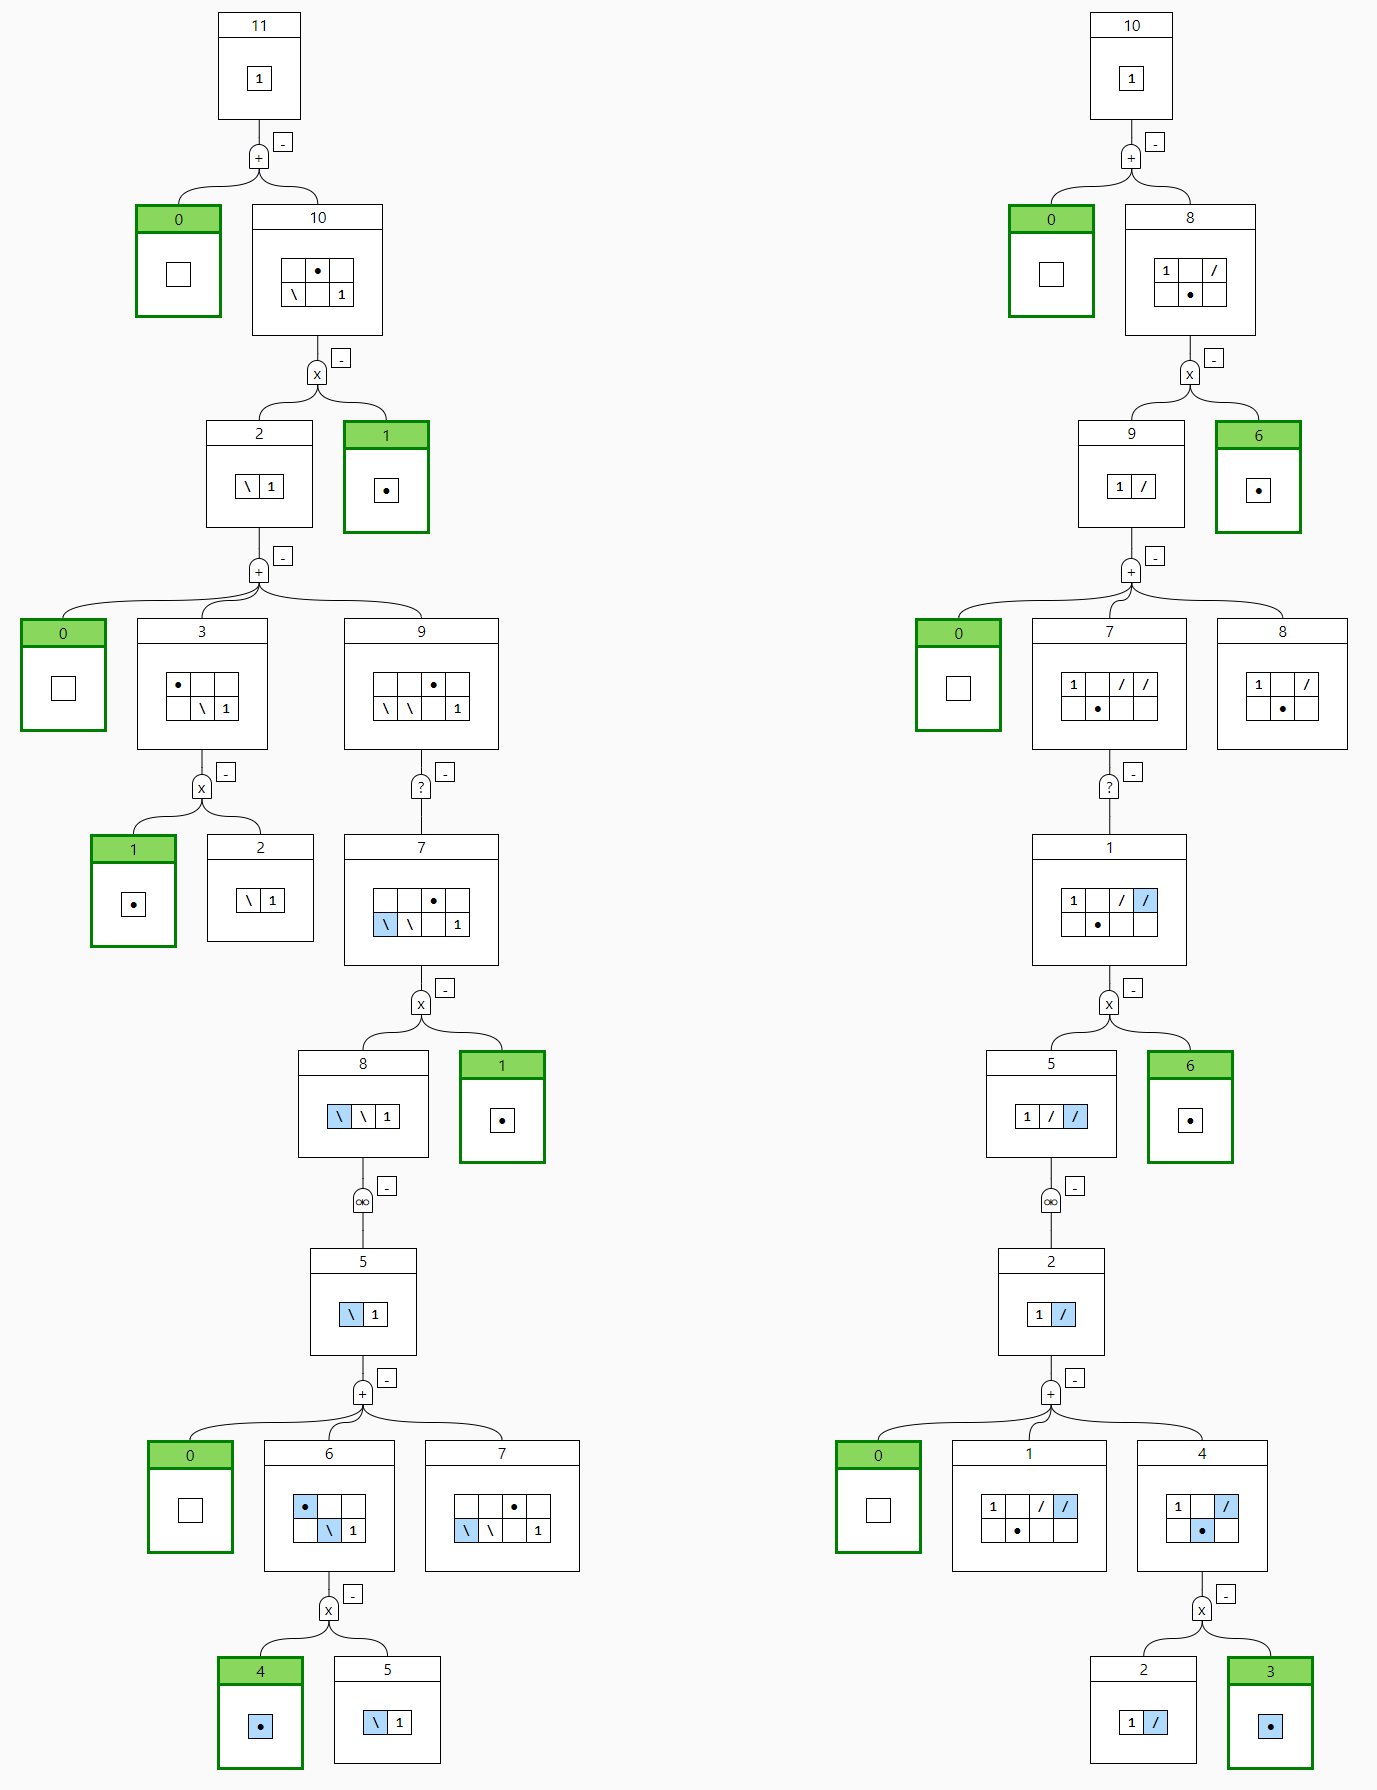
\includegraphics[scale=0.163]{graphics/123_132_specs.png}};
        \caption{Parallel specifications for $\Av{123}$ and $\Av{132}$.}
    \end{figure}
\end{frame}

% Forward steps

\begin{frame}{Parallel bijection - An example for $\Av{123}$ and $\Av{132}$}
    \begin{figure}
        \centering
        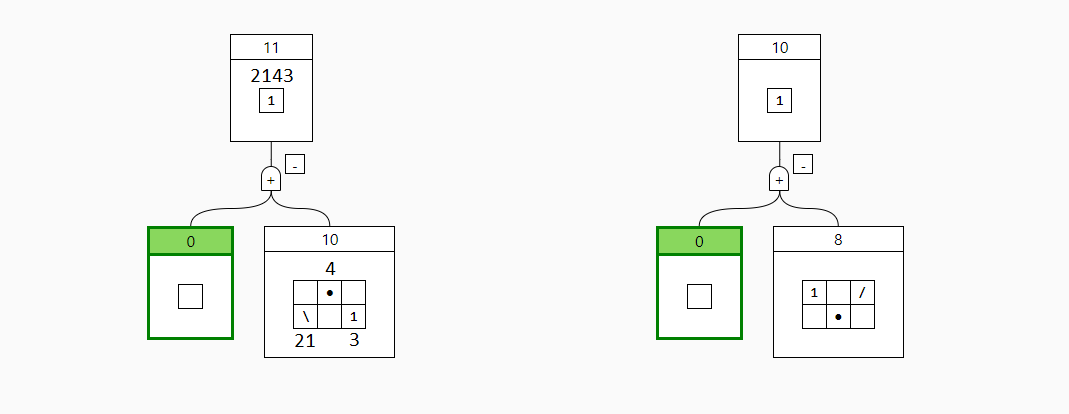
\includegraphics[scale=0.4]{graphics/step01.png}
        \caption{\stepprefix{1}Place topmost point of $2143$ in $\Av{123}$.}
    \end{figure}
\end{frame}

\begin{frame}{Parallel bijection - An example for $\Av{123}$ and $\Av{132}$}
    \begin{figure}
        \centering
        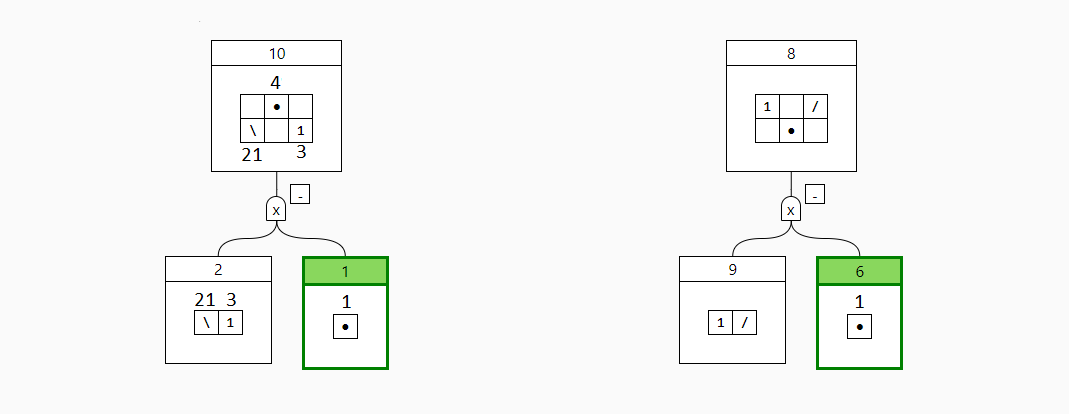
\includegraphics[scale=0.4]{graphics/step02.png}
        \caption{\stepprefix{2}Factor.}
    \end{figure}
\end{frame}


\begin{frame}{Parallel bijection - An example for $\Av{123}$ and $\Av{132}$}
    \begin{figure}
        \centering
        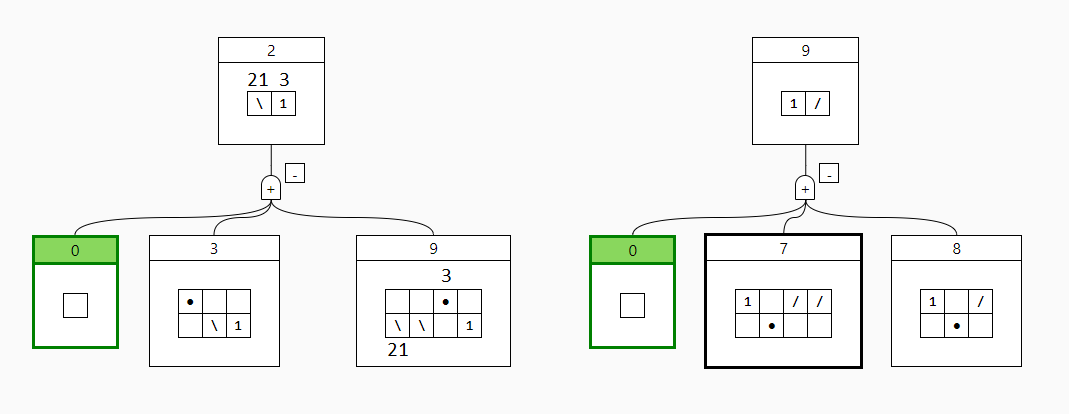
\includegraphics[scale=0.4]{graphics/step03.png}
        \caption{\stepprefix{3}Place topmost in row.}
    \end{figure}
\end{frame}

\begin{frame}{Parallel bijection - An example for $\Av{123}$ and $\Av{132}$}
    \begin{figure}
        \centering
        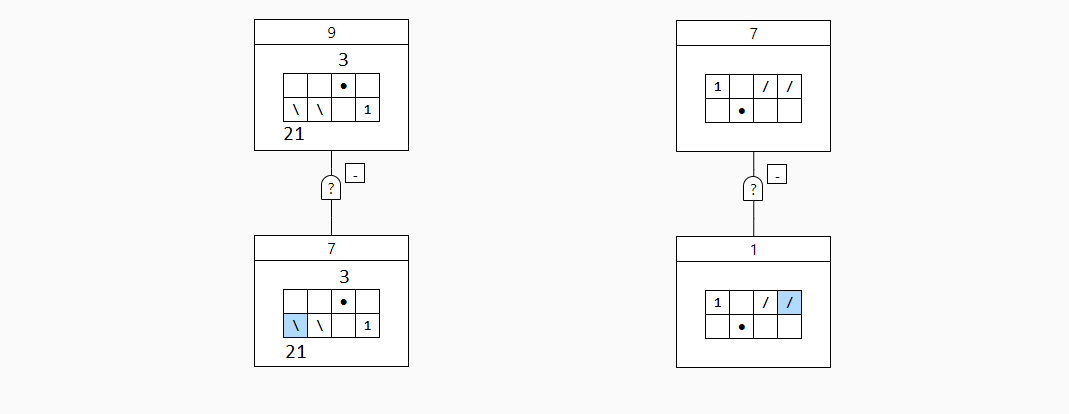
\includegraphics[scale=0.4]{graphics/step04.png}
        \caption{\stepprefix{4}Add assumption in $(0,0)$.}
    \end{figure}
\end{frame}

\begin{frame}{Parallel bijection - An example for $\Av{123}$ and $\Av{132}$}
    \begin{figure}
        \centering
        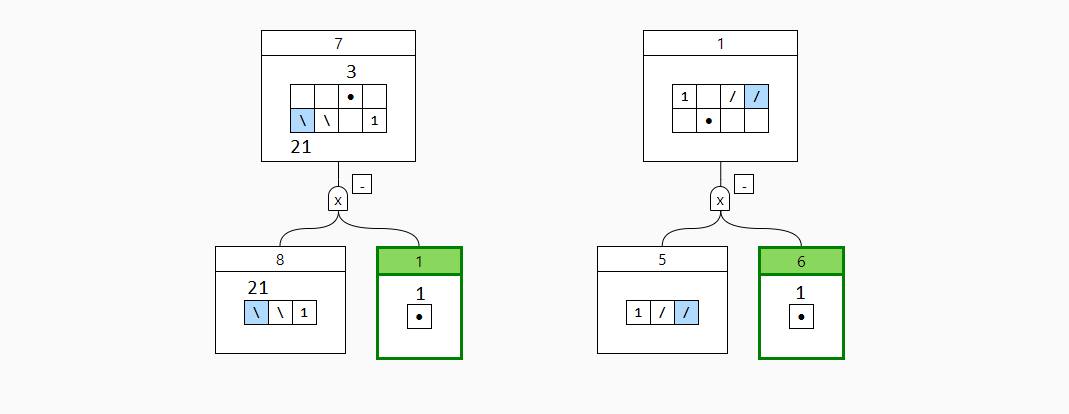
\includegraphics[scale=0.4]{graphics/step05.png}
        \caption{\stepprefix{5}Factor.}
    \end{figure}
\end{frame}


\begin{frame}{Parallel bijection - An example for $\Av{123}$ and $\Av{132}$}
    \begin{figure}
        \centering
        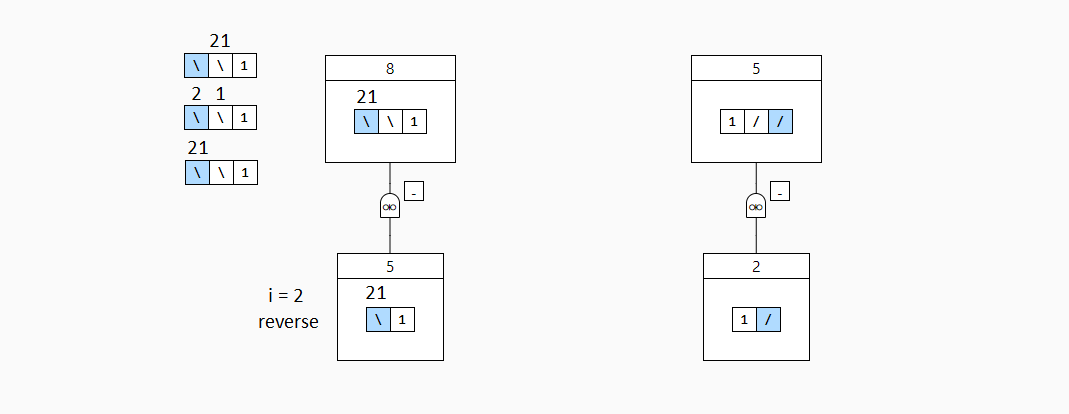
\includegraphics[scale=0.4]{graphics/step06.png}
        \caption{\stepprefix{6}Fuse columns $0$ and $1$.}
    \end{figure}
\end{frame}

\begin{frame}{Parallel bijection - An example for $\Av{123}$ and $\Av{132}$}
    \begin{figure}
        \centering
        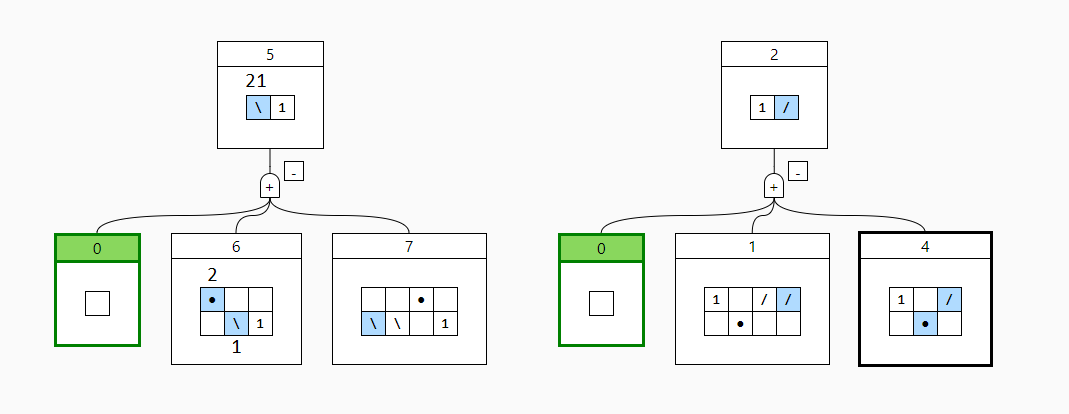
\includegraphics[scale=0.4]{graphics/step07.png}
        \caption{\stepprefix{7}Place topmost in row.}
    \end{figure}
\end{frame}

\begin{frame}{Parallel bijection - An example for $\Av{123}$ and $\Av{132}$}
    \begin{figure}
        \centering
        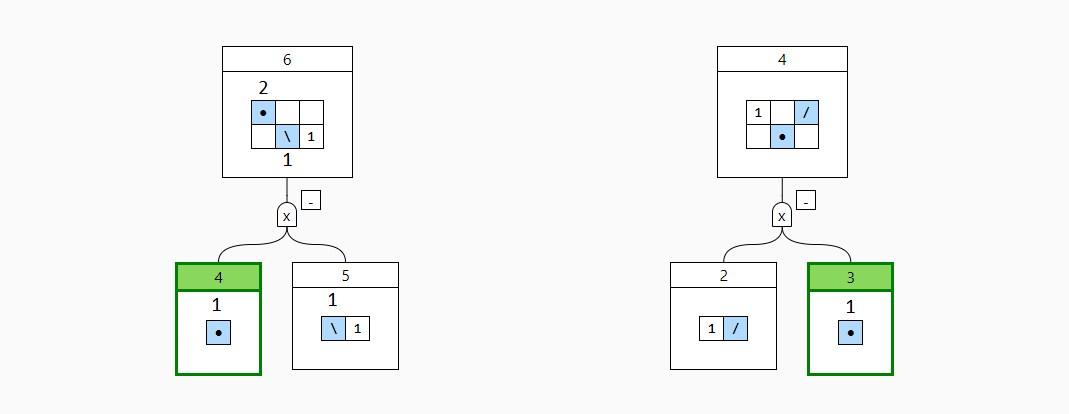
\includegraphics[scale=0.4]{graphics/step08.png}
        \caption{\stepprefix{8}Factor.}
    \end{figure}
\end{frame}

\begin{frame}{Parallel bijection - An example for $\Av{123}$ and $\Av{132}$}
    \begin{figure}
        \centering
        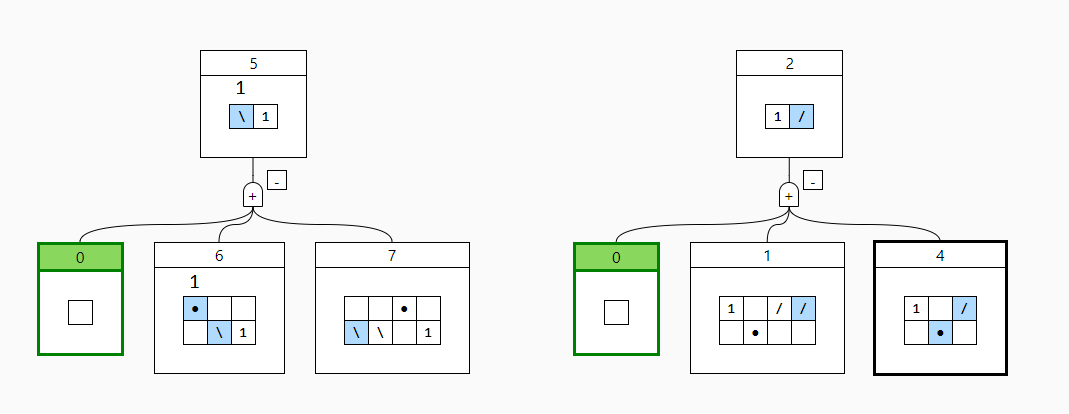
\includegraphics[scale=0.4]{graphics/step09.png}
        \caption{\stepprefix{9}Place topmost in row.}
    \end{figure}
\end{frame}

\begin{frame}{Parallel bijection - An example for $\Av{123}$ and $\Av{132}$}
    \begin{figure}
        \centering
        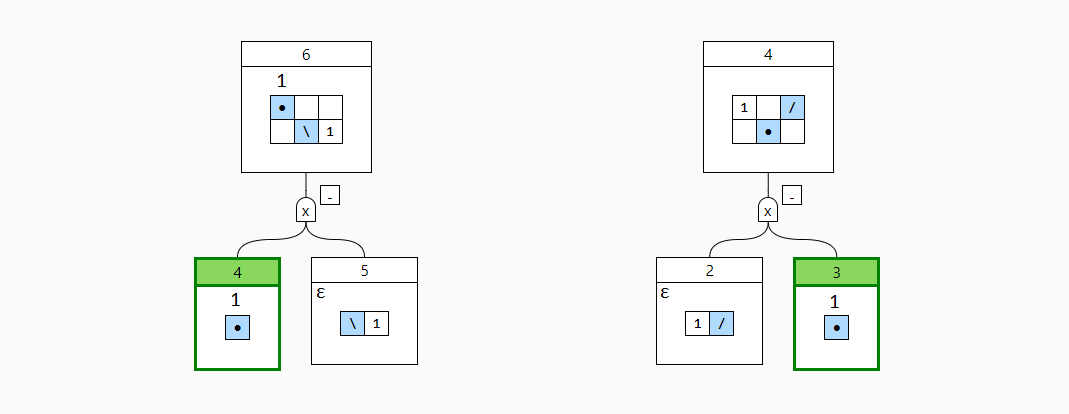
\includegraphics[scale=0.4]{graphics/step10.png}
        \caption{\stepprefix{10}Factor.}
    \end{figure}
\end{frame}

% Parse trees

\begin{frame}{Parallel bijection - An example for $\Av{123}$ and $\Av{132}$}
    %The parse tree we have created for $\Av{132}$.
    \begin{figure}
        \centering
        \tikz{\draw [black, opacity=0] (0,0) rectangle (10,7.5);}
        \only<1>{%
            \tikz [remember picture,overlay] \node at ([yshift=-.25cm,xshift=0cm]current page.center) {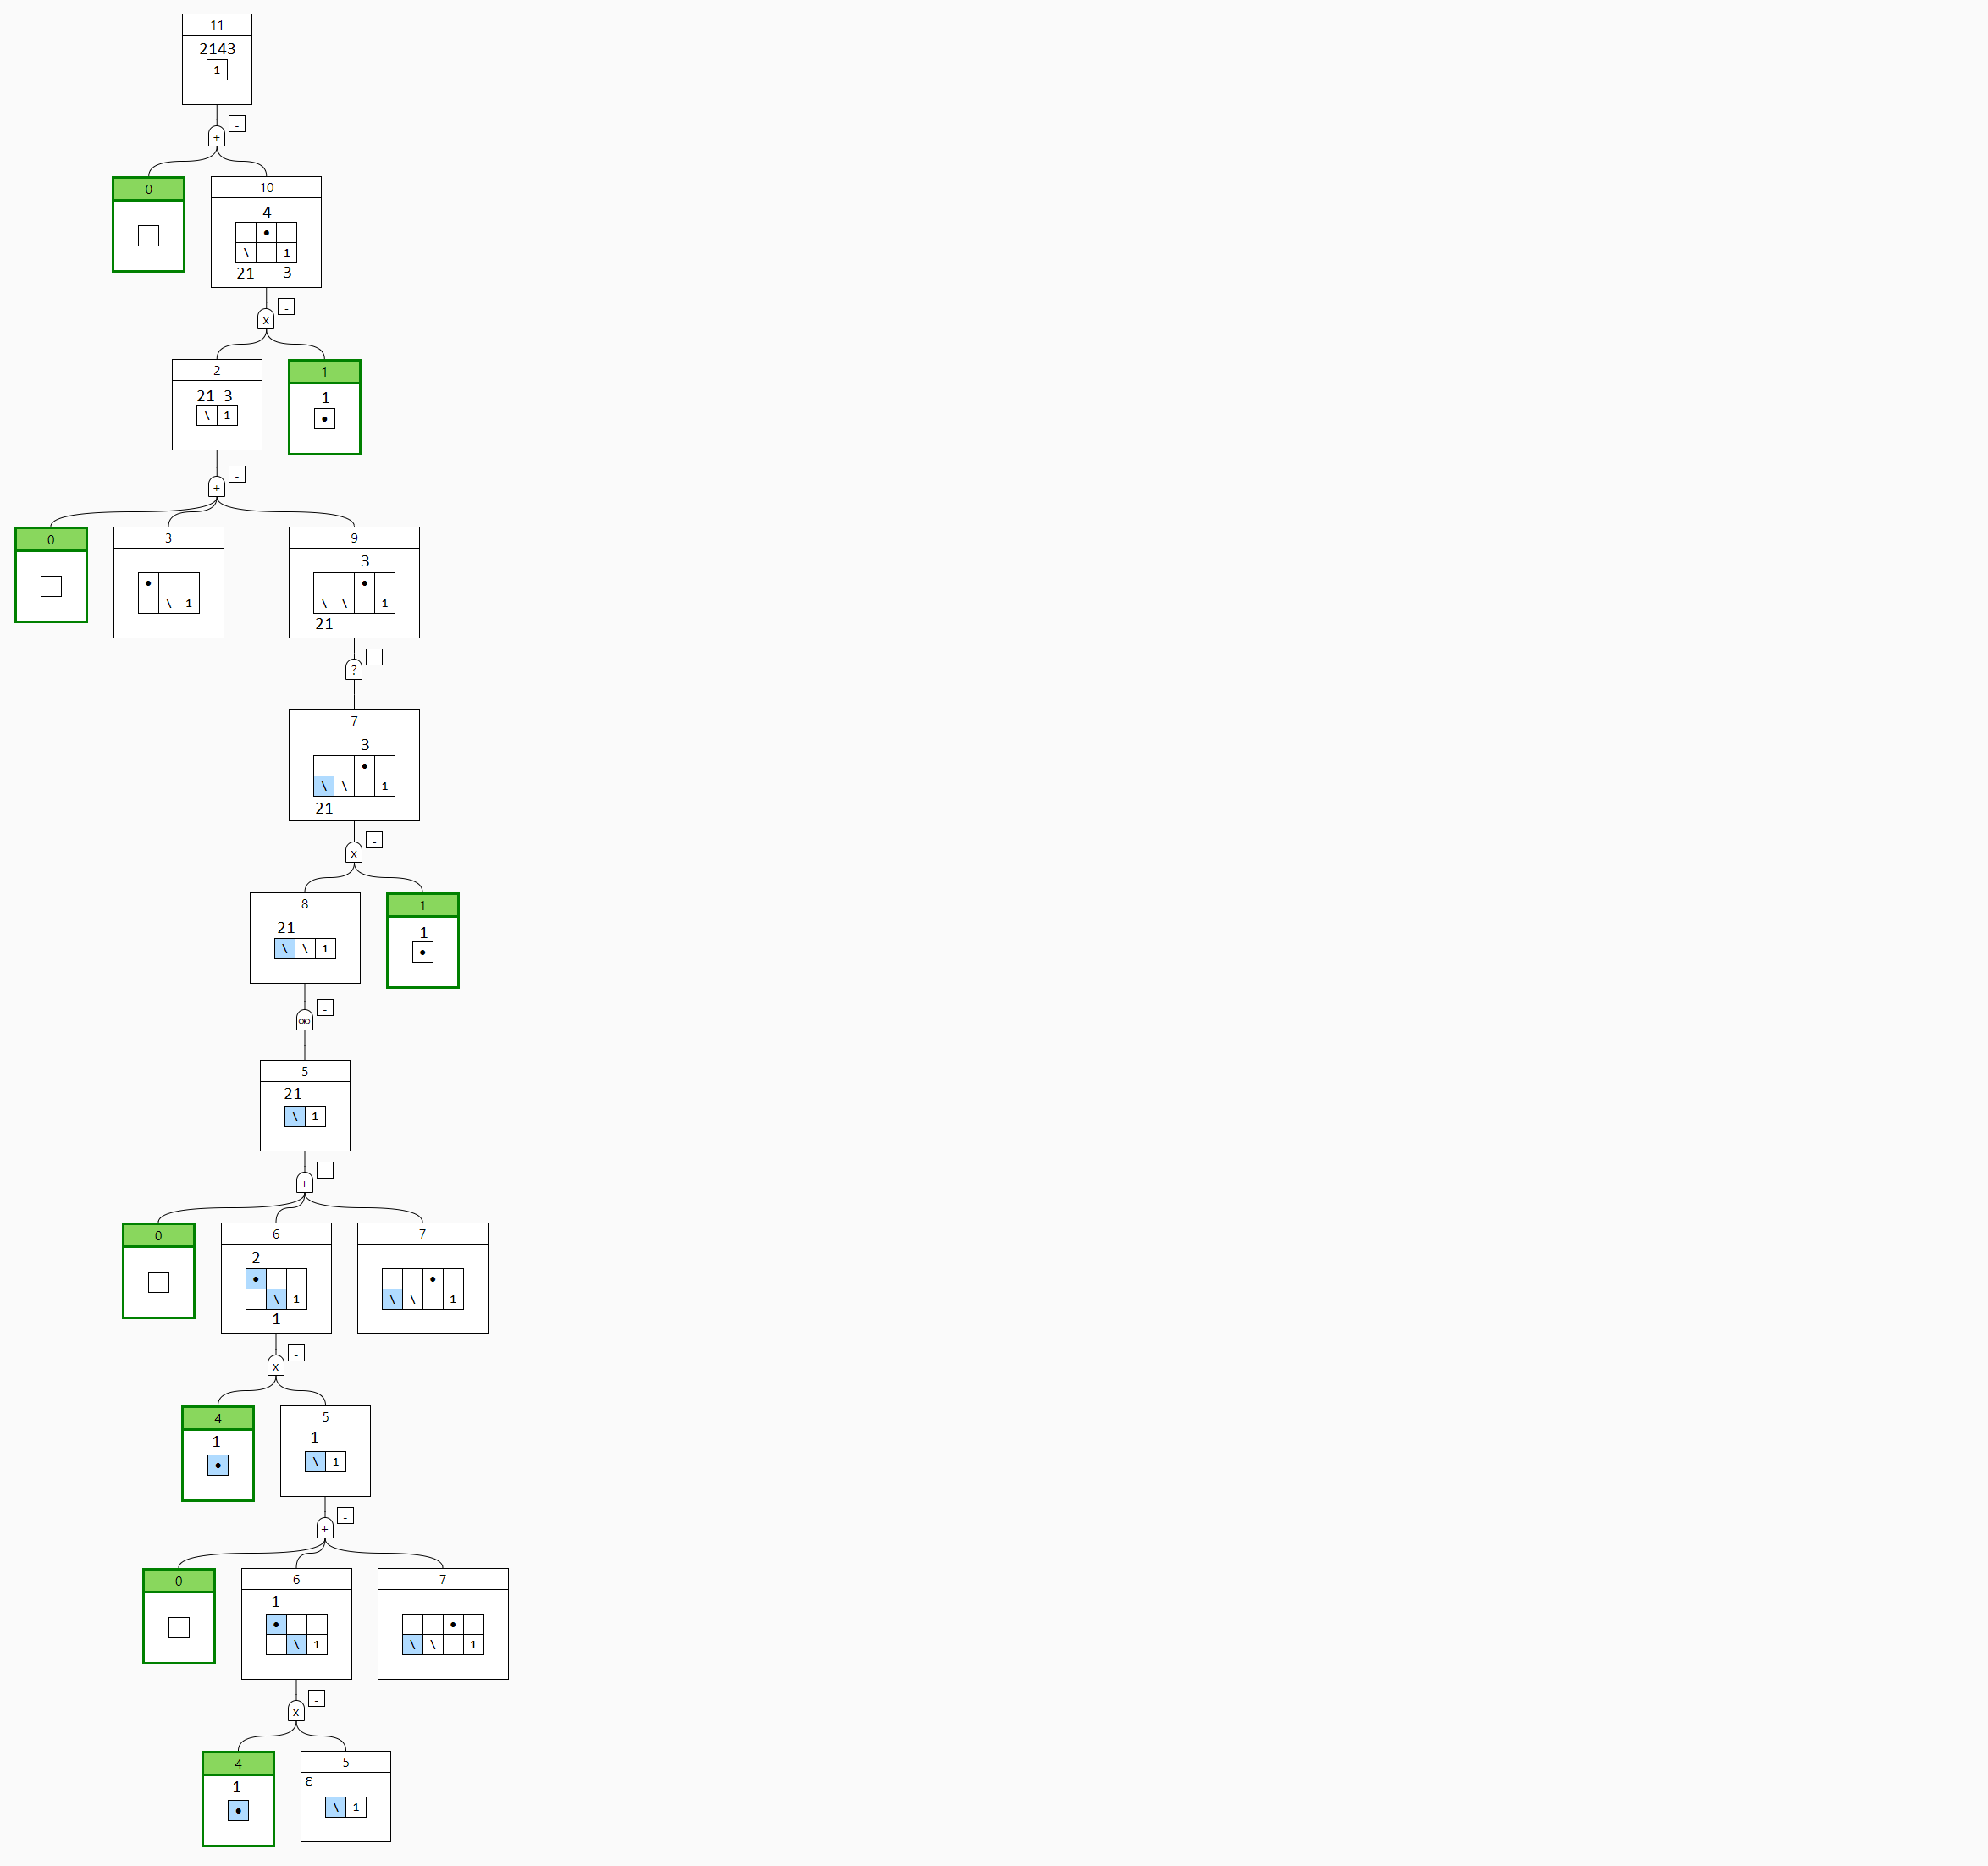
\includegraphics[scale=0.12]{graphics/parse_trees_01.png}};
        }
        \only<2>{%
            \tikz [remember picture,overlay] \node at ([yshift=-.25cm,xshift=0cm]current page.center) {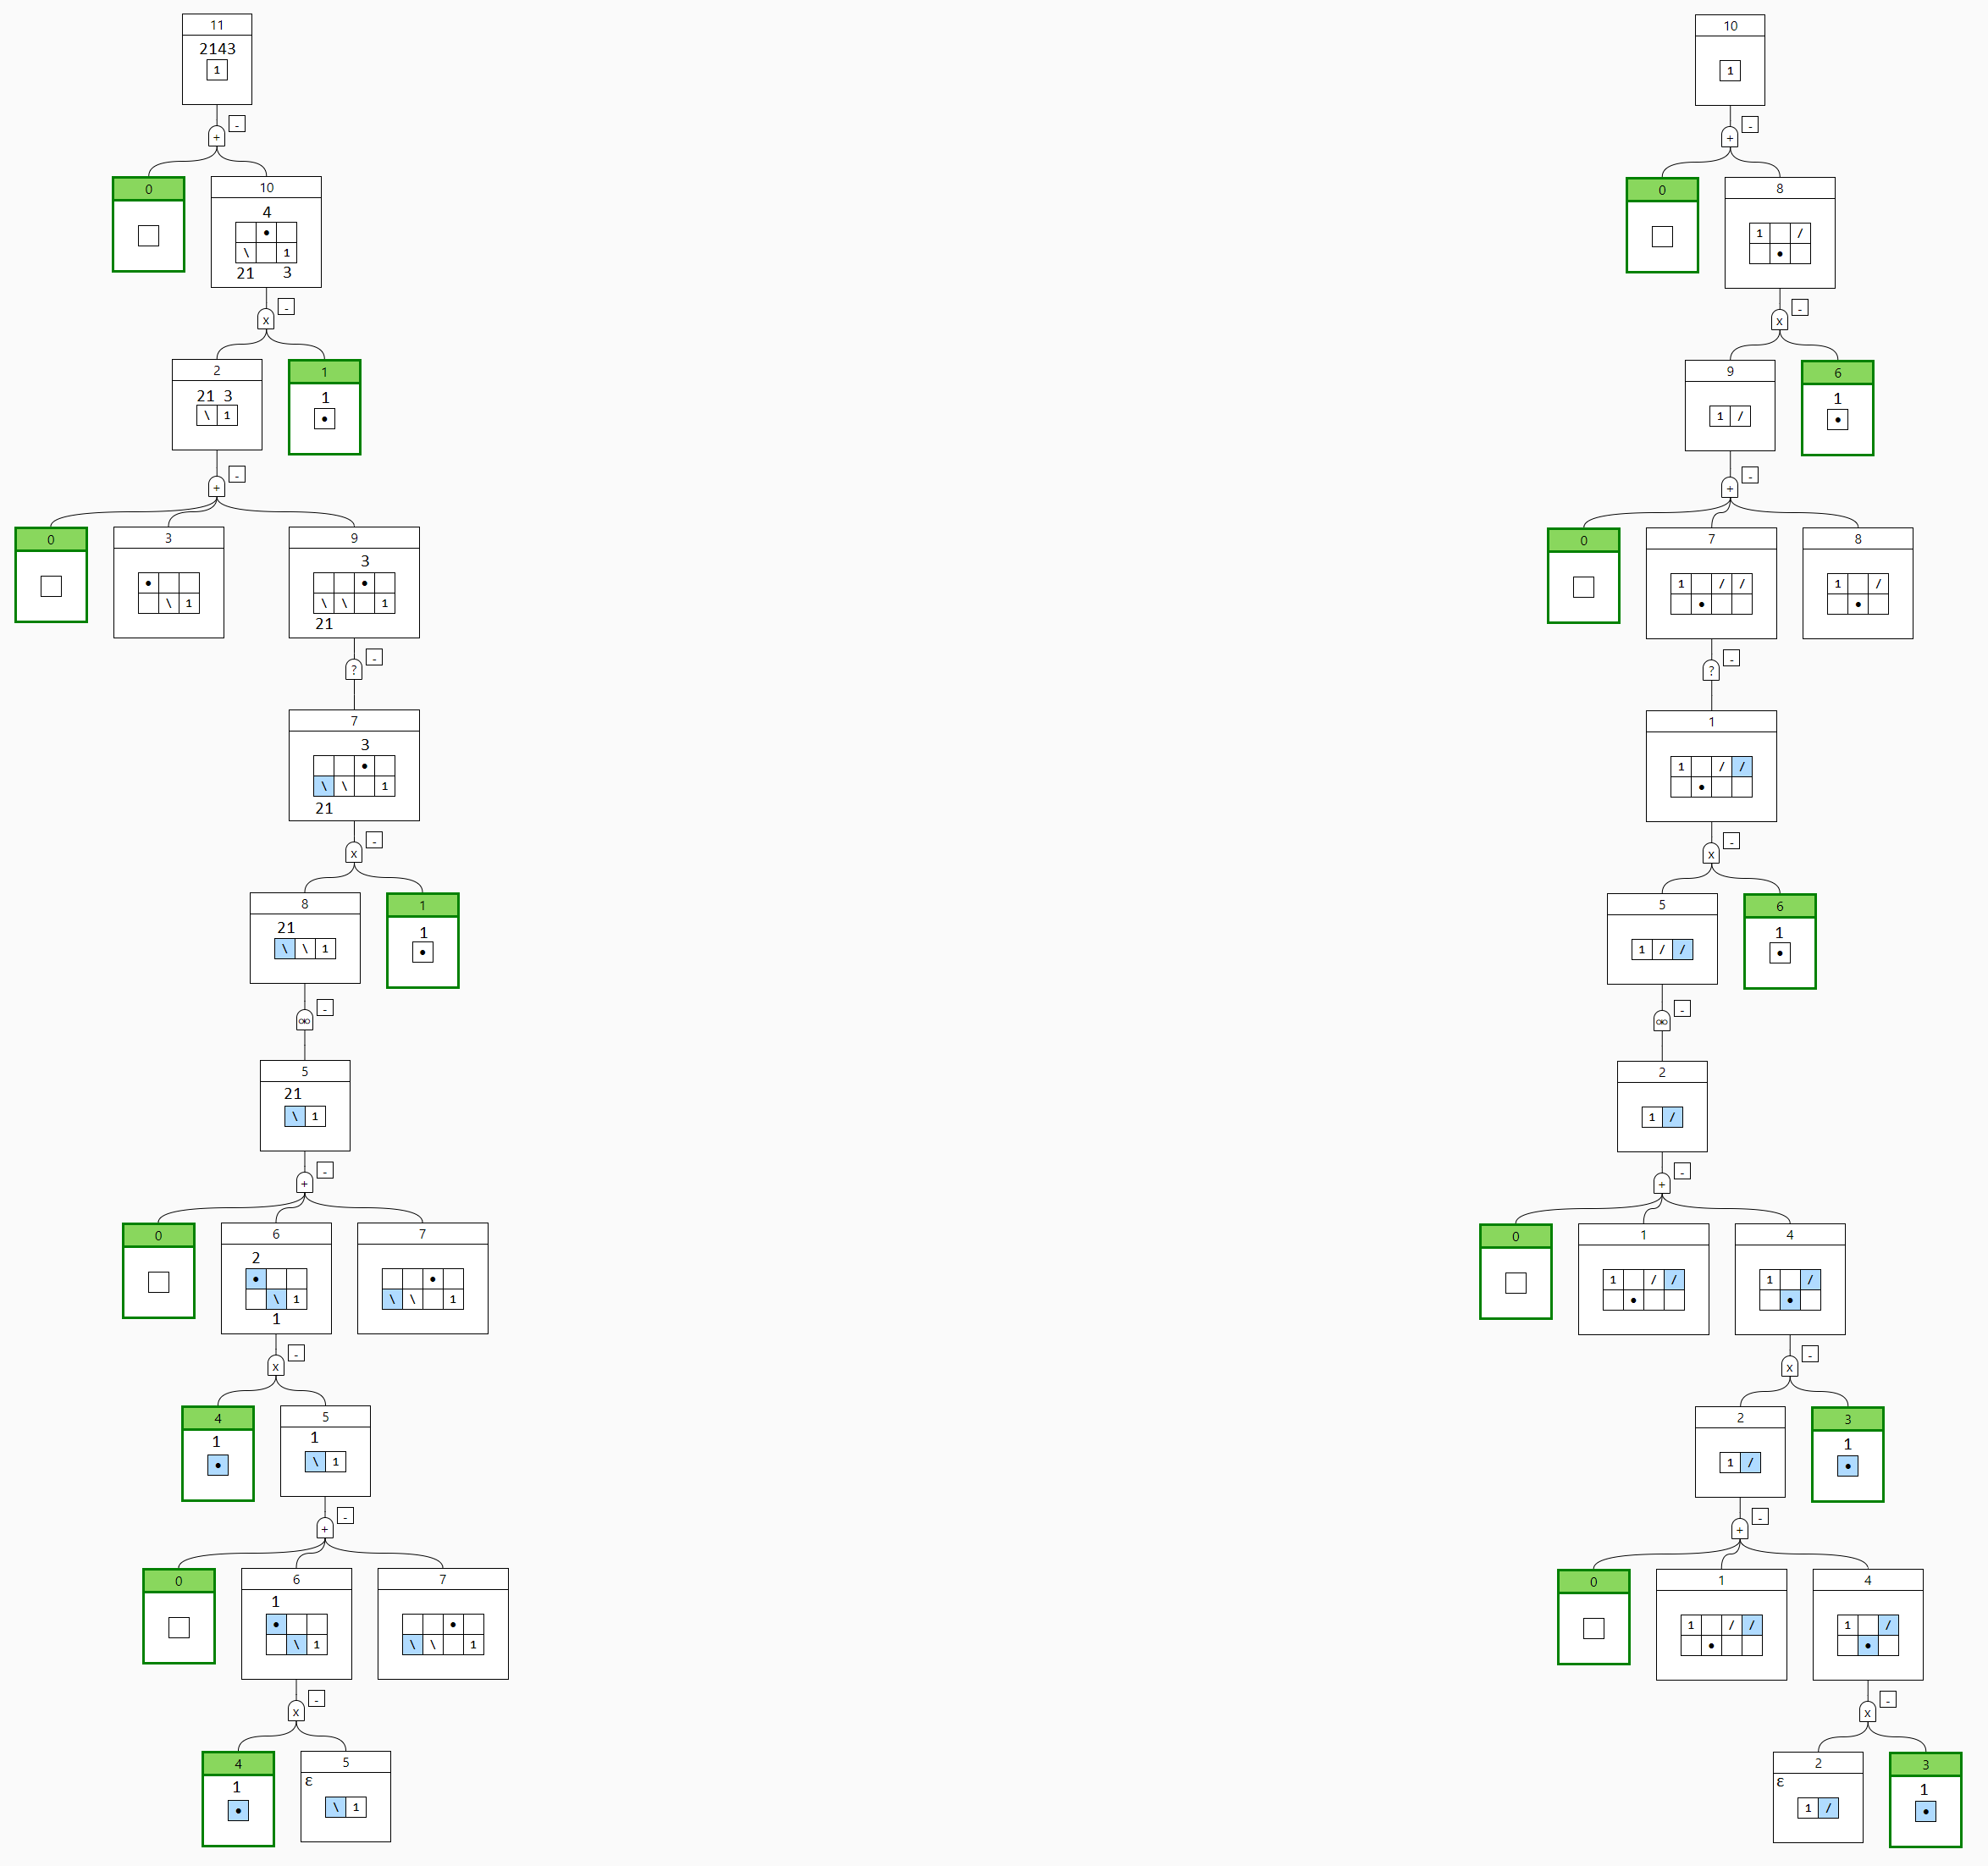
\includegraphics[scale=0.12]{graphics/parse_trees_02.png}};
        }
        \only<3>{%
            \tikz [remember picture,overlay] \node at ([yshift=-.25cm,xshift=0cm]current page.center) {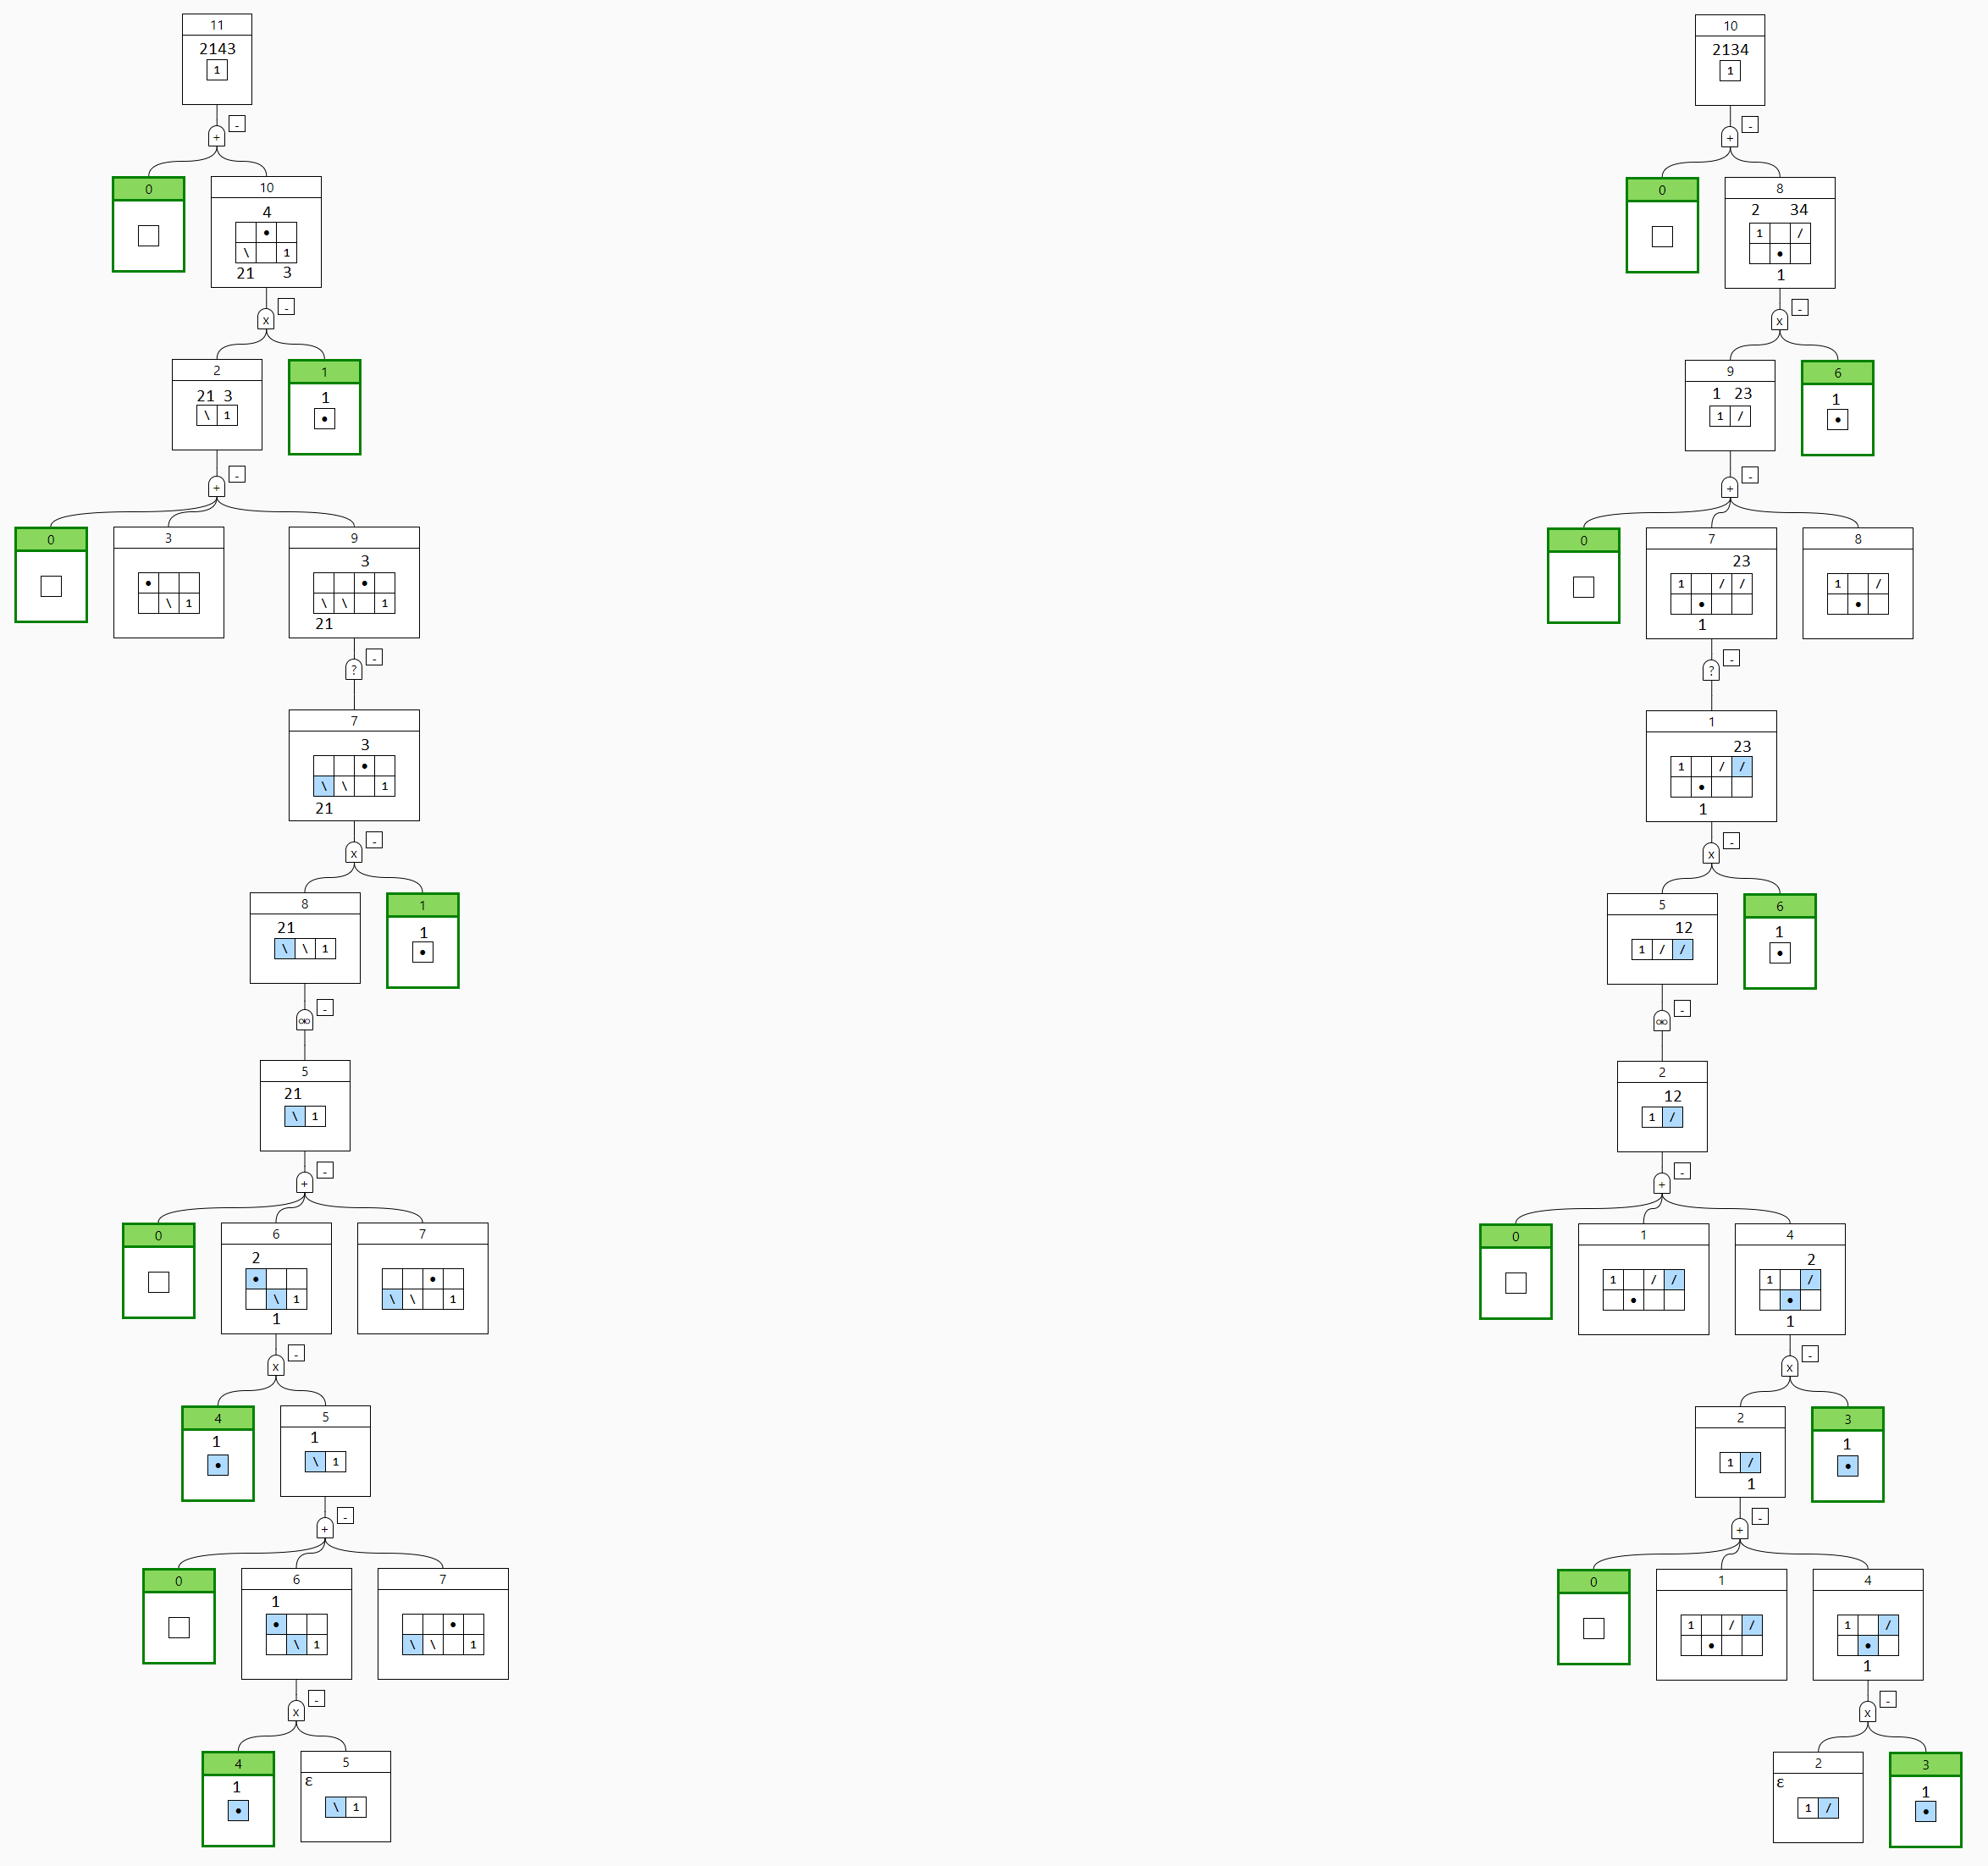
\includegraphics[scale=0.12]{graphics/parse_trees_03.png}};
        }
        \only<4>{%
            \tikz [remember picture,overlay] \node at ([yshift=-.25cm,xshift=0cm]current page.center) {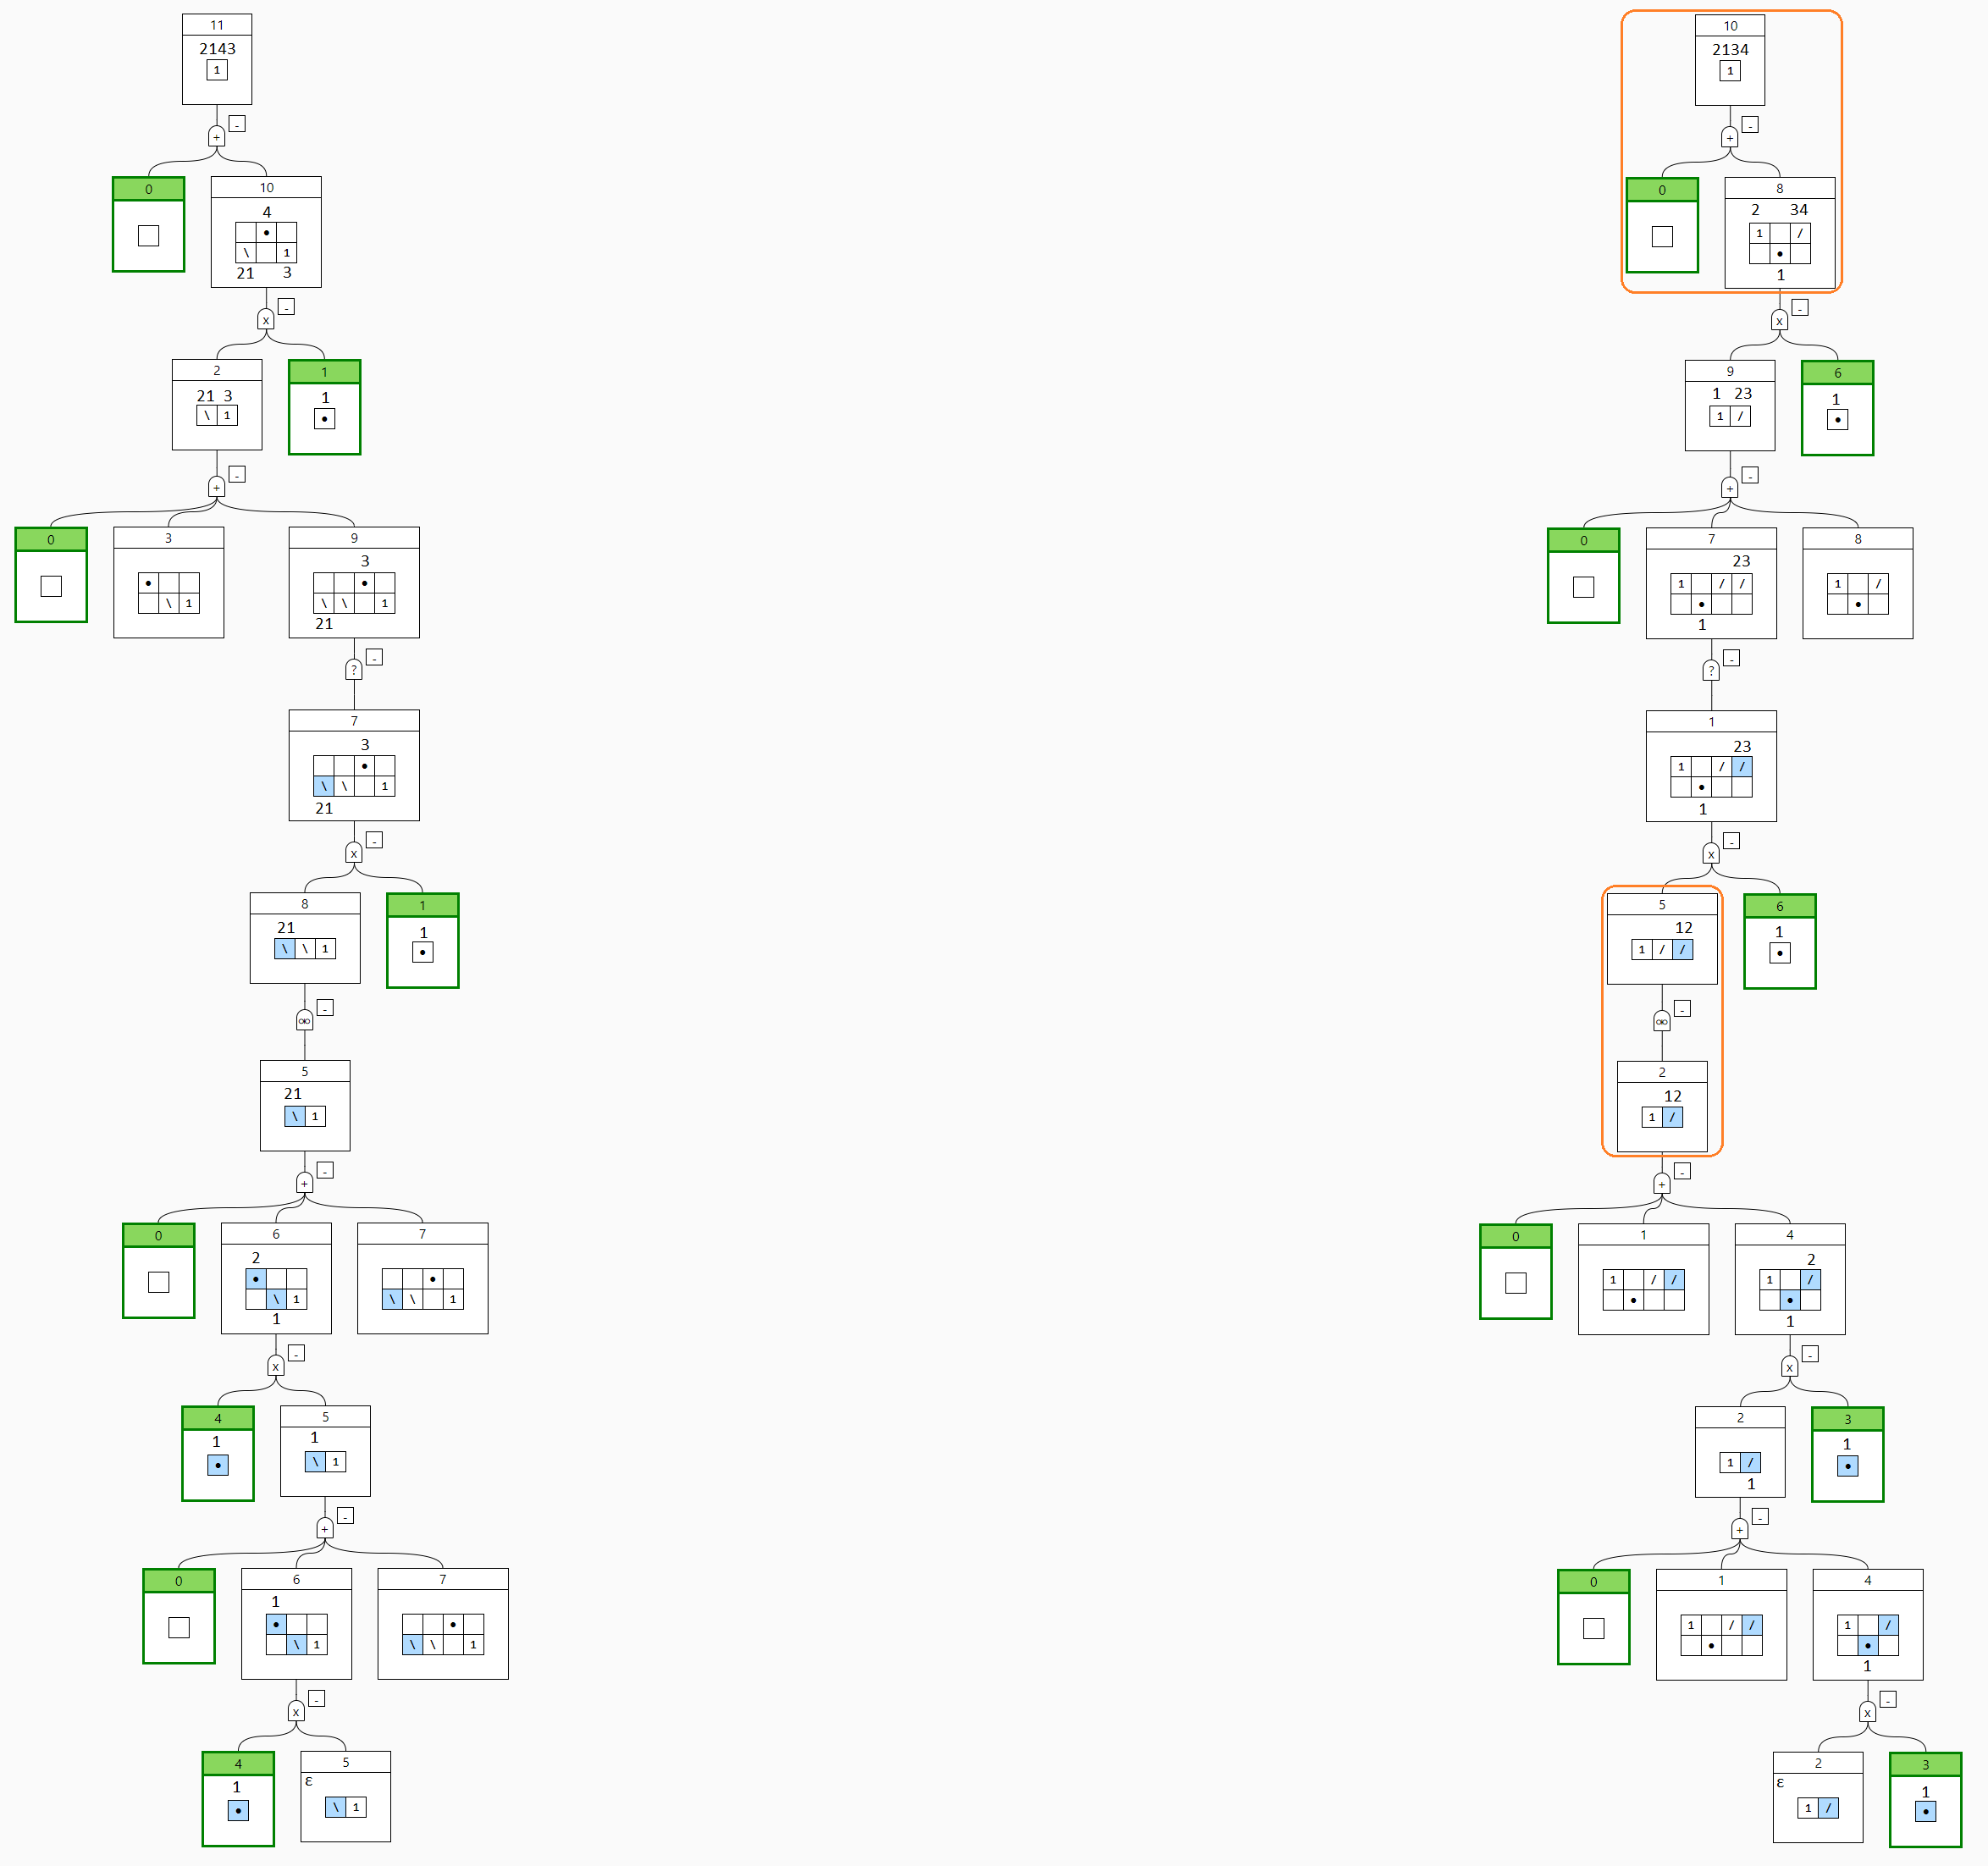
\includegraphics[scale=0.12]{graphics/parse_trees_04.png}};
        }
        %\onslide<2->
    \end{figure}
\end{frame}

% Backward

\begin{frame}{Parallel bijection - An example for $\Av{123}$ and $\Av{132}$}
    \begin{figure}
        \centering
        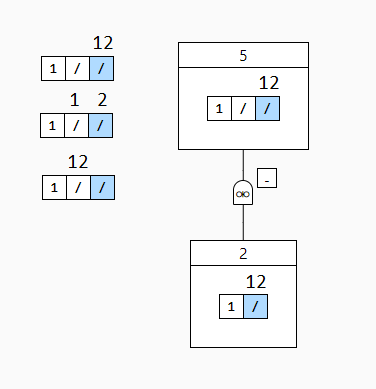
\includegraphics[scale=0.4]{graphics/fus_back.png}
        \caption{Backward step for fusion.}
    \end{figure}
\end{frame}
\begin{frame}{Parallel bijection - An example for $\Av{123}$ and $\Av{132}$}
    Final step
    \begin{figure}
        \centering
        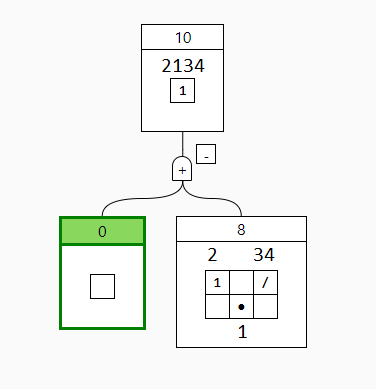
\includegraphics[scale=0.4]{graphics/final_parse.png}
        \caption{Final step.}
    \end{figure}
\end{frame}


\section{Bijection Search}
\begin{frame}{Bijection search}
    \begin{itemize}
        \item Expands both universes until both contain specifications
        \item Gathers all the matched pairs
        \item Uses dynamic programming and backtracking
        \item A second tree search attempts to construct parallel specifications from matched pairs
        \item Detects false positives from recursion
    \end{itemize}
    \onslide<2>{%
    \begin{figure}
        \centering
        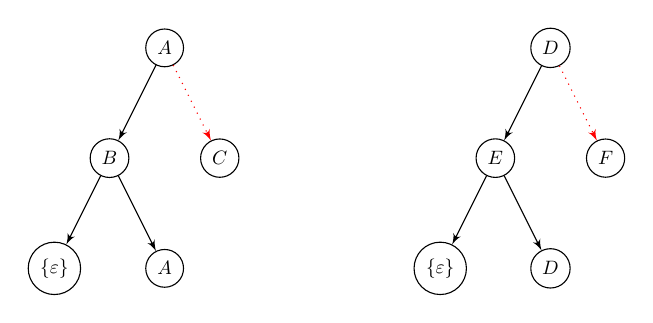
\begin{tikzpicture}[vertex/.style = {shape=circle,draw,minimum size=1.5em},edge/.style = {->,> = latex'},scale=0.7, every node/.style={scale=0.7}]
\node[vertex] (a) at (0,0) {$A$};
\node[vertex] (b) at (-1,-2) {$B$};
\node[vertex] (c) at (1,-2) {$C$};
\node[vertex] (d) at (-2,-4) {$\set{\varepsilon}$};
\node[vertex] (e) at (0,-4) {$A$};

\draw[edge] (a) to (b);
\draw[edge, red, dotted] (a) to (c);
\draw[edge] (b) to (d);
\draw[edge] (b) to (e);

\node[vertex] (f) at (7,0) {$D$};
\node[vertex] (g) at (6,-2) {$E$};
\node[vertex] (h) at (8,-2) {$F$};
\node[vertex] (i) at (5,-4) {$\set{\varepsilon}$};
\node[vertex] (j) at (7,-4) {$D$};

\draw[edge] (f) to (g);
\draw[edge, red, dotted] (f) to (h);
\draw[edge] (g) to (i);
\draw[edge] (g) to (j);
\end{tikzpicture}
        \caption{Classes $B$ and $E$ are incorrectly matched because of a recursion to $A$ and $D$ that we fail to matched later.}
    \end{figure}
    }
\end{frame}
%\begin{frame}{Modifications for fusion and catalytic variables}
    \begin{itemize}
        \item Catalytic variables in both cells require BFS to decide on reversing
        \item Equivalence labels can contain nonequivalent classes and required partial specification extraction during the search
        \item Catalytic variables were labelled when added to know which reached higher up the tree.
    \end{itemize}
\end{frame}

\section{Results}
\begin{frame}{Results}
    \begin{itemize}
        \item Cross domain bijections
            \subitems{%
                \item Words and permutations
            }
        \item Known Wilf classes
        \item Experimental classes
            \subitems{%
                \item $11 \times 4$
                \item $10 \times 4$
                \item $9 \times 4$ (except one class)
            }
    \end{itemize}
\end{frame}
\begin{frame}{A bijection between words and permutations}
    \begin{itemize}
    \item $\Av{231,312,321}$
    \[1, 1, 2, 3, 5, 8, 13, 21, 34, 55, 89, \dotsc\]
    \item Binary strings avoiding $11$
    \[1, 2, 3, 5, 8, 13, 21, 34, 55, 89, 144, \dotsc\]
    \end{itemize}
    \begin{figure}
        \centering
        {
\newcommand{\nodeA}{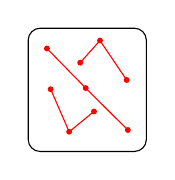
\begin{tikzpicture}[scale=1*0.5, every node/.style={scale=1}]
    \def\xscale{0.5} % Horizontal scale factor
    \def\yscale{0.5} % Vertical scale factor
    \def\spnt{0.075} % Size of smaller points
    \def\lpnt{0.125} % Size of larger points
    \def\roundscale{0.5} % The rounding factor
    \draw[rounded corners=2ex*\roundscale] (0,0) rectangle (6.0*\xscale,6.26*\yscale);
    \fill[red] (2.64*\xscale, 4.51*\yscale) circle (\spnt);
    \fill[red] (3.645242338035261*\xscale, 5.634518213709113*\yscale) circle (\spnt);
    \fill[red] (5.0*\xscale, 3.63*\yscale) circle (\spnt);
    \draw[red] (2.64*\xscale, 4.51*\yscale) -- (3.645242338035261*\xscale,5.634518213709113*\yscale) -- (5.0*\xscale,3.63*\yscale);
    \fill[red] (1.14*\xscale, 3.16*\yscale) circle (\spnt);
    \fill[red] (2.08*\xscale, 1.0*\yscale) circle (\spnt);
    \fill[red] (3.34*\xscale, 2.03*\yscale) circle (\spnt);
    \draw[red] (1.14*\xscale, 3.16*\yscale) -- (2.08*\xscale,1.0*\yscale) -- (3.34*\xscale,2.03*\yscale);
    \fill[red] (0.95*\xscale, 5.23*\yscale) circle (\spnt);
    \fill[red] (2.92*\xscale, 3.22*\yscale) circle (\spnt);
    \fill[red] (5.06*\xscale, 1.09*\yscale) circle (\spnt);
    \draw[red] (0.95*\xscale, 5.23*\yscale) -- (2.92*\xscale,3.22*\yscale) -- (5.06*\xscale,1.09*\yscale);
\end{tikzpicture}}
\newcommand{\nodeB}{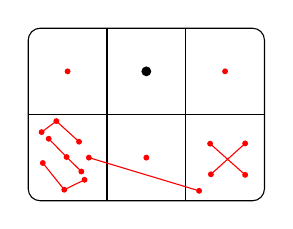
\begin{tikzpicture}[scale=1*0.5, every node/.style={scale=1}]
    \def\xscale{1.0} % Horizontal scale factor
    \def\yscale{0.7} % Vertical scale factor
    \def\spnt{0.075} % Size of smaller points
    \def\lpnt{0.125} % Size of larger points
    \def\roundscale{0.5} % The rounding factor
    \fill[red] (1.0*\xscale,4.695*\yscale) circle (\spnt);
    \fill[red] (3.0*\xscale,1.565*\yscale) circle (\spnt);
    \fill[red] (5.0*\xscale,4.695*\yscale) circle (\spnt);
    \draw[rounded corners=2ex*\roundscale] (0,0) rectangle (6.0*\xscale,6.26*\yscale);
    \draw (2.0*\xscale, 6.26*\yscale) -- (2.0*\xscale, 0);
    \draw (4.0*\xscale, 6.26*\yscale) -- (4.0*\xscale, 0);
    \draw (0, 3.13*\yscale) -- (6.0*\xscale, 3.13*\yscale);
    \fill[red] (4.64*\xscale, 0.96*\yscale) circle (\spnt);
    \fill[red] (5.51*\xscale, 2.08*\yscale) circle (\spnt);
    \draw[red] (4.64*\xscale, 0.96*\yscale) -- (5.51*\xscale,2.08*\yscale);
    \fill[red] (1.54*\xscale, 1.56500*\yscale) circle (\spnt);
    \fill[red] (4.34*\xscale, 0.36*\yscale) circle (\spnt);
    \draw[red] (1.54*\xscale, 1.56500*\yscale) -- (4.34*\xscale,0.36*\yscale);
    \fill[red] (4.62*\xscale, 2.07*\yscale) circle (\spnt);
    \fill[red] (5.51*\xscale, 0.94*\yscale) circle (\spnt);
    \draw[red] (4.62*\xscale, 2.07*\yscale) -- (5.51*\xscale,0.94*\yscale);
    \fill[red] (0.34*\xscale, 2.49*\yscale) circle (\spnt);
    \fill[red] (0.7137700370786788*\xscale, 2.8907811732342776*\yscale) circle (\spnt);
    \fill[red] (1.29*\xscale, 2.1410793034814266*\yscale) circle (\spnt);
    \draw[red] (0.34*\xscale, 2.49*\yscale) -- (0.7137700370786788*\xscale,2.8907811732342776*\yscale) -- (1.29*\xscale,2.1410793034814266*\yscale);
    \fill[red] (0.37*\xscale, 1.37*\yscale) circle (\spnt);
    \fill[red] (0.9155476869638484*\xscale, 0.3994524095796065*\yscale) circle (\spnt);
    \fill[red] (1.43*\xscale, 0.76*\yscale) circle (\spnt);
    \draw[red] (0.37*\xscale, 1.37*\yscale) -- (0.9155476869638484*\xscale,0.3994524095796065*\yscale) -- (1.43*\xscale,0.76*\yscale);
    \fill[red] (0.52*\xscale, 2.25*\yscale) circle (\spnt);
    \fill[red] (0.974077815720099*\xscale, 1.5866958340474693*\yscale) circle (\spnt);
    \fill[red] (1.35*\xscale, 1.06*\yscale) circle (\spnt);
    \draw[red] (0.52*\xscale, 2.25*\yscale) -- (0.974077815720099*\xscale,1.5866958340474693*\yscale) -- (1.35*\xscale,1.06*\yscale);
    \fill (3*\xscale,4.69500*\yscale) circle (\lpnt);
\end{tikzpicture}}
\newcommand{\nodeD}{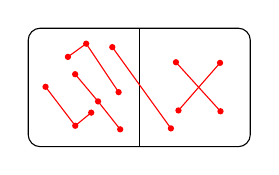
\begin{tikzpicture}[scale=0.4, every node/.style={scale=1}]
        \def\xscale{1.0} % Horizontal scale factor
        \def\yscale{1.0} % Vertical scale factor
        \def\spnt{0.1} % Size of smaller points
        \def\lpnt{0.125} % Size of larger points
        \def\roundscale{0.5} % The rounding factor
        \draw[rounded corners=2ex*\roundscale] (0,0) rectangle (7.05*\xscale,3.76*\yscale);
        \draw (3.525*\xscale, 3.76*\yscale) -- (3.525*\xscale, 0);
        \fill[red] (4.77*\xscale, 1.15*\yscale) circle (\spnt);
        \fill[red] (6.09*\xscale, 2.66*\yscale) circle (\spnt);
        \draw[red] (4.77*\xscale, 1.15*\yscale) -- (6.09*\xscale,2.66*\yscale);
        \fill[red] (2.67*\xscale, 3.16*\yscale) circle (\spnt);
        \fill[red] (4.53*\xscale, 0.58*\yscale) circle (\spnt);
        \draw[red] (2.67*\xscale, 3.16*\yscale) -- (4.53*\xscale,0.58*\yscale);
        \fill[red] (4.69*\xscale, 2.68*\yscale) circle (\spnt);
        \fill[red] (6.103901218159451*\xscale, 1.1230608594818354*\yscale) circle (\spnt);
        \draw[red] (4.69*\xscale, 2.68*\yscale) -- (6.103901218159451*\xscale,1.1230608594818354*\yscale);
        \fill[red] (1.26*\xscale, 2.85*\yscale) circle (\spnt);
        \fill[red] (1.84*\xscale, 3.27*\yscale) circle (\spnt);
        \fill[red] (2.87*\xscale, 1.73*\yscale) circle (\spnt);
        \draw[red] (1.26*\xscale, 2.85*\yscale) -- (1.84*\xscale,3.27*\yscale) -- (2.87*\xscale,1.73*\yscale);
        \fill[red] (0.55*\xscale, 1.9*\yscale) circle (\spnt);
        \fill[red] (1.4930670970674682*\xscale, 0.6636520415041379*\yscale) circle (\spnt);
        \fill[red] (2.0*\xscale, 1.08*\yscale) circle (\spnt);
        \draw[red] (0.55*\xscale, 1.9*\yscale) -- (1.4930670970674682*\xscale,0.6636520415041379*\yscale) -- (2.0*\xscale,1.08*\yscale);
        \fill[red] (1.49*\xscale, 2.3*\yscale) circle (\spnt);
        \fill[red] (2.2169083602620874*\xscale, 1.4365892987622655*\yscale) circle (\spnt);
        \fill[red] (2.92*\xscale, 0.55*\yscale) circle (\spnt);
        \draw[red] (1.49*\xscale, 2.3*\yscale) -- (2.2169083602620874*\xscale,1.4365892987622655*\yscale) -- (2.92*\xscale,0.55*\yscale);
\end{tikzpicture}}
\begin{tikzpicture}
\fill[opacity=0] (-0.8,-1.2) rectangle (9.1,2.2);
\end{tikzpicture}
\begin{tikzpicture}[overlay,xshift=-9.25cm,yshift=1.15cm]
\draw<2-> (0,1) node {\tiny $1,1,2,3,5,\ldots$};
\node<2-> (a) at (0,0) {\nodeA};
\draw<3-> (3.5,2.25) node {\tiny $0,1,2,3,5,\ldots$};
\node<3-> (b) at (3.5,1) {\nodeB};
\node<3-> (c) at (3.5,-1)  {$\varepsilon$};
\node<4-> (e) at (7.5,2)  {\tikz{\fill (0,0) circle (0.1);}};
\draw<4-> (7.5,1) node {\tiny $1,2,3,5,8,\ldots$};
\node<4-> (d) at (7.5,0)  {\nodeD};

\draw<3-> (a) -- (b);
\draw<3-> (a) -- (c);
\draw<4-> (b) -- (d);
\draw<4-> (b) -- (e);

\draw<5->[orange!70] (6,-0.85) rectangle (9,0.85);
\end{tikzpicture}
}
        \onslide<5->{\caption{The class that is isomorphic to the binary strings.}}
    \end{figure}
\end{frame}
\begin{frame}{Known Wilf classes}
    \begin{itemize}
        \item<1-> Classes avoiding one, two or three patterns of size $3$.
            \subitems{%
                \item All classes in \authcite{simionandschmidt}.
                \item The bijection we found for $\Av{123}$ and $\Av{132}$ seems to agree with theirs.
            }
        \item<2-> Classes avoiding one pattern of size $3$ and one of size $4$.
        \item<3-> $\Av{1234}$, $\Av{1243}$ and $\Av{1432}$.
        \subitems{%
            \item $\Av{2143}$ is missing.
        }
    \end{itemize}
\end{frame}
\begin{frame}{Known Wilf classes, $\Av{1234}$ and $\Av{1243}$}
    \begin{figure}
        \tikz{\draw [black, opacity=0] (0,0) rectangle (10,7.5);}
        \tikz [remember picture,overlay] \node at ([yshift=-.25cm,xshift=0cm]current page.center) {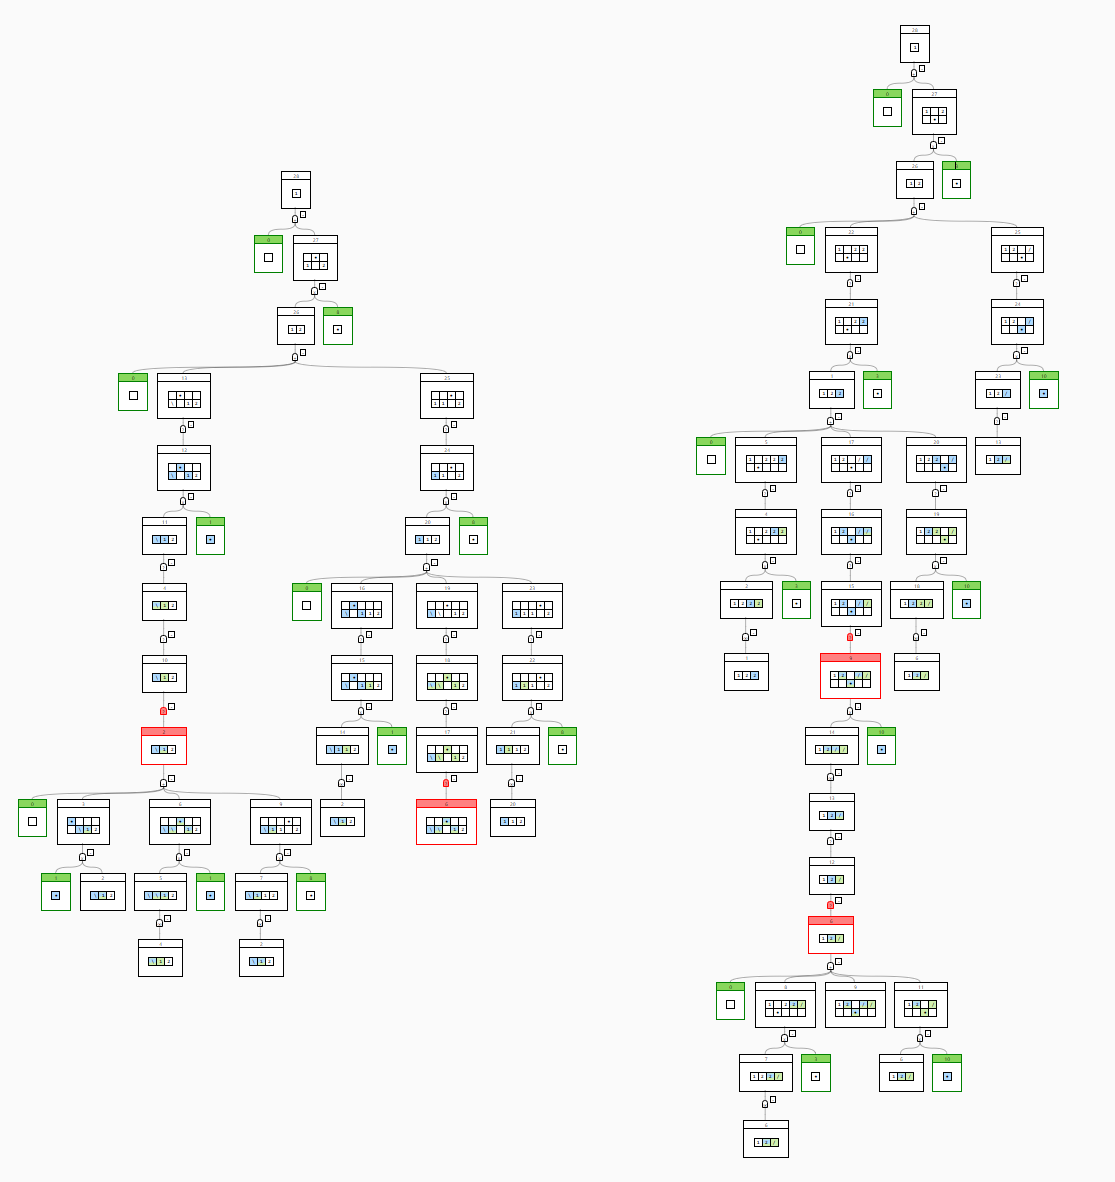
\includegraphics[scale=0.25]{graphics/1234_1243.png}};
        \caption{The parallel specifications found for $\Av{1234}$ and $\Av{1243}$.}
    \end{figure}
\end{frame}
\begin{frame}{Experimental classes}
    \begin{enumerate}
    \only<1>{\item $\Av{1243,1342,1423,1432,2143,2413,3142,3412,4231}$}
    \only<2>{{\color{red} \item $\Av{1243,1342,1423,1432,2143,2413,3142,3412,4231}$}}
    \item $\Av{1243,1342,1423,1432,2413,2431,3142,3412,4231}$
    \item $\Av{1243,1342,1423,2143,2413,2431,3142,3412,4231}$
    \item $\Av{1243,1342,1432,2143,2413,2431,3142,3412,4231}$
    \item $\Av{1243,1342,2143,2413,2431,3142,3412,4132,4231}$
    \item $\Av{1324,1342,2143,2341,2413,2431,3142,3241,3412}$
    \end{enumerate}
    \onslide<2->{\begin{figure}
        \centering
        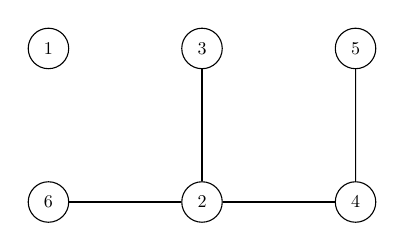
\begin{tikzpicture}[vertex/.style = {shape=circle,draw,minimum size=2.25em},scale=0.65, every node/.style={scale=0.65}]
    \node[vertex] (c1) at (-3,3) {$1$};
    \node[vertex] (c2) at (0,0) {$2$};
    \node[vertex] (c3) at (0,3) {$3$};
    \node[vertex] (c4) at (3,0) {$4$};
    \node[vertex] (c5) at (3,3) {$5$};
    \node[vertex] (c6) at (-3,0) {$6$};
    \draw (c2) -- (c3);
    \draw (c2) -- (c4);
    \draw (c2) -- (c6);
    \draw (c4) -- (c5);
\end{tikzpicture}
        \caption{The bijections found for an experimental class.}
    \end{figure}}
\end{frame}

\section{Conclusion}
\begin{frame}{Conclusion and future work}
    \begin{itemize}
        \item First fully automatic bijections (that we know of).
        \item Offers structural insight.
        \item Discover equivalence rules.
        \item Use a search specifically for bijections.
        \item Continue classifying $n \times 4$ for $n < 9$.
    \end{itemize}
    \onslide<2->{\centering \Huge Thanks for listening\\Questions?}
\end{frame}

\begin{frame}[allowframebreaks]
    \printbibliography{}
\end{frame}

\end{document}